% /* GRASP: Copyright 1997,1998,1999  Bruce Allen */
% $Id: man_inspiral.tex,v 1.42 1999/09/29 19:44:41 ballen Exp $
\section{GRASP Routines: Gravitational Radiation from Binary Inspiral}
\label{s:inspiral}
\setcounter{equation}0
One of the principal sources of gravitational radiation which should be
detectable with the first or second generation of interferometric
detectors is {\it binary inspiral}.  This radiation is produced by a
pair of massive and compact orbiting objects, such as neutron stars or
black holes.

The simplest case is when the two objects are describing a circular
orbit about their common center-of-mass, and neither object is spinning
about its own axis.  With these assumptions the system is then
described, at any time, by the masses $m_1$ and $m_2$ of the objects,
and their orbital frequency $\Omega$.  (It is also necessary to
describe the orientation of the orbital plane and the positions of the
masses at a given time; these are details we will sort out later).

For convenience in dealing with dimensional quantities, we introduce
the {\it Solar Mass} $M_\odot$ and the {\it Solar Time} $T_\odot$
defined by
\begin{eqnarray}
M_\odot &=& 1.989 \times 10^{33} \> {\rm grams}\\
\label{e:tsolar}
T_\odot &=& \left( {G \over c^3} \right) M_\odot = 4.925491 \times
10^{-6} \> {\rm sec}.
\end{eqnarray}
GRASP functions typically measure masses in units of $M_\odot$ and
times in units of seconds.
\clearpage

\subsection{Chirp generation routines}
\setcounter{equation}0
The next several subsections document a number of routines 
for generating ``chirps'' from coalescing binaries.  
This package of routines is intended to be versatile, flexible and robust; 
and yet still fairly simple to use.
The implementation we have included in this package is based
on the second post-Newtonian treatment of binary inspiral presented in
\cite{biww} and augmented by the spin-orbit and spin-spin corrections
presented in \cite{willwiseman} and 2.5 post-Newtonian
order corrections in \cite{blanchet:1996}.
The notation we use -- even in the source code  --
closely reflects the notation used in those papers.
In keeping with that notation, these routines calculate
the {\bf orbital phase} and {\bf orbital frequency}. 
The gravitational-wave phase of the dominant quadrupolar radiation
can be obtained by multiplying the orbital phase by two.
The routines can be used to compute a few 
chirp waveforms (say to make transparencies for a seminar),
or for wholesale computations of a bank of matched filters.

All of the chirp generation routines, 
in particular the ubiquitous {\tt make\_filters()}, 
compute what has come to be
known as {\bf  ``restricted'' post-Newtonian chirps}.
This means they include all post-Newtonian corrections
(up to the specified order)
in the phase evolution, but only the dominant quadrupole
amplitude.

The routines are flexible in the sense that they have a number
of {\it run-time} options available for choosing the post-Newtonian
order of the phase calculations, or choosing whether or not
to include spin effects.
We have also isolated those parts of the code where the messy
post-Newtonian coefficients appear;
thus the routines may be
easily modified to include yet higher-order post-Newtonian terms as
they become available.

The post-Newtonian equations for the orbital phase evolution are
notoriously ill-behaved \cite{cutleretal,lincolnwill} as the binary
system nears coalescence.  In this regime the expansion parameters
[namely the relative velocity $v/c$ of the bodies and/or the field
strength $GM_{\rm tot}/(c^2 r_{orbit})$] used in the derivation are
comparable to unity.  In post$^2$-Newtonian calculations higher orders
such as post$^3$-Newtonian terms have been discarded.  Because of this
truncation, quantities that are are positive definite in an exact
calculation (say the energy-loss rate, or the time derivative of the
orbital frequency) often become negative in their post-Newtonian
expansion when the orbital separation becomes small.  When this happens
you are using a post-Newtonian expression in a regime where its
validity is questionable.  This is cause for concern, and it may be
cause for terminating a chirp calculation; but, it need not crash your
code.  A full-scale gravitational-wave search will need to compute
chirps over a broad range of parameters, virtually assuring that any
post-Newtonian chirp generator will be pushed into a region of
parameter space where it doesn't belong.  These routines are designed
to traverse these dangerous regions of parameter space as well as
possible and gently warn the user of the dangers encountered.  The
calling routines may wish to act on the warnings coming from the chirp
generator.  For example a severe warning may prompt the calling routine
to discard a given filter from  a data search, because the second
post-Newtonian calculation of the chirp is so dubious that it can't
give meaningful results.

In the next several sections we detail the use of three routines used
to compute the ``chirp'' of a coalescing binary system.  The first
routine we describe is {\tt phase\_frequency()}.  This is the
underlying routine for the other chirp routines.  Given a set of
parameters ({\it e.g.} the two masses, and the upper and lower cut-off
frequency for the chirp) it returns the orbital phase and orbital
frequency evolution as a function of time.  Next we describe {\tt
chirp\_filter()} which returns two (unnormalized) chirp signals.  This
routine can be used for wholesale production of a bank of templates for
a coalescing binary search.  
%The routine {\tt strain()} returns the
%full second post-Newtonian gravitational wave strain.  This can be used
%for plotting and examining the expected waveform of a given coalescing
%binary, or to add a ``realistic'' signal into detector noise.  The
%strain output contains all the (sub)harmonic structure and its
%amplitude reflects the true astrophysical distance to the source.

\clearpage

\subsection{Function: {\tt phase\_frequency()}}
\label{ss:phase_frequency}
\setcounter{equation}0
{\tt
int phase\_frequency(float m1, float m2, float spin1, float spin2, int n\_phaseterms,
   float *phaseterms, float Initial\_Freq, float Max\_Freq\_Rqst,
   float *Max\_Freq\_Actual, float Sample\_Time, float **phase, float **frequency,
   int *steps\_alloc, int *steps\_filld, int err\_cd\_sprs)
}\\
This function computes the {\bf orbital  phase} 
and {\bf orbital frequency} evolution of
an inspiraling binary. It returns an integer termination code
indicating how and why the chirp calculation terminated.
This routine is the engine that powers the other chirp generation
routines.
The arguments are:
\begin{description}
\item{\tt m1}: Input.  The mass of body-1 in solar masses.
\item{\tt m2}: Input.  The mass of body-2 in solar masses.
\item{\tt spin1}: Input.  The dimensionless spin parameter 
  of body-1. See section on spin effects.
\item{\tt spin2}: Input.  The dimensionless spin parameter 
  of body-2. See section on spin effects.
\item{\tt n\_phaseterms}: Input. Integer describing
 the number of post-Newtonian (pN) approximation terms implemented in
 the phase and frequency calculations. In the present implementation
 this should be set to $5$.
\item{\tt phaseterms}: Input. The array 
  {\tt phase\_terms[0..n\_phaseterms-1]} specifies which pN
  approximation terms will be included in the phase frequency
  calculations.  Setting  {\tt phase\_terms[i]=0.0} nullifys the term.
  Setting  {\tt phase\_terms[i]=1.0} includes the term.  This allows
  for easy run-time nullification of any term in the phase and
  frequency evolution, {\it e.g.} setting {\tt phase\_terms[4]=0.0}
  eliminates the {\it second} post-Newtonian terms from the
  calculation.
\item{\tt Initial\_Freq}: Input.  The starting orbital frequency of the
  chirp in Hz.
\item{\tt Max\_Freq\_Rqst}: Input.  The requested orbital frequency
  where the chirp will stop. However, the actual calculation
  may not proceed all the way to this orbital frequency.  This is 
  discussed at length below.
\item{\tt Max\_Freq\_Actual}: Output. The floating 
  number {\tt *Max\_Freq\_Actual}
  is the orbital frequency in Hz where the chirp actually terminated.
\item{\tt Sample\_Time}: Input.  The time interval between successive samples,
  in seconds.
\item{\tt phase}: Input/Output. The phase ephemeris $\Omega$ in radians
  is stored in the array {\tt *phase[0..steps\_filld-1]}.
  Input in the sense that much of the internal logic of 
  {\tt  phase\_frequency()} depends on how the pointers {\tt *phase}
  (and {\tt *frequency} below) are set.
  If either is set to {\tt NULL} memory allocation will be performed
  inside  {\tt  phase\_frequency()}. If both are not {\tt NULL}
  then it is assumed the calling routine has allocated the memory
  before calling  {\tt  phase\_frequency()}.
\item{\tt frequency}: Input/Output. Similar to {\tt phase} above.
  The frequency ephemeris $f=d\Omega/dt$ is stored in the array 
  {\tt *frequency[0..steps\_filld-1]}.
\item{\tt steps\_alloc}: Input/Output. The integer
  {\tt *steps\_alloc} is the number of floating point entries
  allocated for storing the 
  phase and frequency evolution, {\it i.e.} the length of
  {\tt **phase} and {\tt **frequency}.
  This integer should be set in the calling
  routine if memory is allocated there,
  or it will be set inside {\tt  phase\_frequency()} if memory
  is to be allocated there.
  If both of the pointers {\tt *phase} and {\tt *frequency} are
  not {\tt NULL} then {\tt  phase\_frequency()} understands that
  the calling routine is taking responsibility
  for allocating the memory for the chirp, and the calling routine
  must set {\tt *steps\_alloc} accordingly. 
  In this case {\tt phase\_frequency()} will
  fill up the  arrays  {\tt **phase} and {\tt **frequency} until the memory
  is full ({\it i.e} fill them with {\tt *steps\_alloc} of floats)
  or until the chirp terminates, whichever is less.
\item{\tt steps\_filld}: Output. The integer {\tt *steps\_filld}
  is the integer number of time steps actually computed
  for this evolution. It is less than or equal to {\tt *steps\_alloc}.
\item{\tt clscnc\_time}: Output. The float {\tt *clscnc\_time}
 is the time to coalescence in seconds,
 measured from the instant when the orbital frequency is 
 {\tt Initial\_Freq} given by $t_c$ in Eqs.(\ref{e:frequencyns})
 and (\ref{e:phasens}).
\item{\tt err\_cd\_sprs}: Input. Error code suppression.
 This integer determines
 at what level of disaster encountered in the computation 
 of the chirp the user will be explicitly warned about
 with a printed message.
 Set to {\tt 0}: prints all the termination
 messages. Set to {\tt 4000}: suppresses
 all but a few messages which are  harbingers of complete disaster.
 The termination messages are numbered from 0 to 3999 
 loosely in accordance with their severity
 (the larger numbers corresponding to more severe warnings). 
 Any message with a number less than {\tt err\_cd\_sprs} will not
 be printed.
 A termination code of 0 means the chirp calculation was executed
 as requested.
 A termination code in the 1000's means the chirp was terminated
 early because the post-Newtonian approximation was deemed no longer
 valid.
 A termination code in the 2000's generally indicates some problem with
 memory allocation.
 A termination code in the 3000's generally indicates a serious logic fault.
 Many of these ``3000'' errors result in the termination of the routine.
 If you get an error message number it is easy to find the portion of 
 source code where the fault occurred; just do a character string search
 on the four digit number.
 
\end{description}

This phase and frequency generator has a number of very specialized features 
which will be discussed later. 
However,
before we proceed further, we show a simple example of how  
{\tt phase\_frequency()} can be used.

\begin{description}
\item{Authors:} Alan Wiseman, agw@tapir.caltech.edu and Bruce Allen, ballen@dirac.phys.uwm.edu
\item{Comments:}
This function will need to be extended when results of order 2.5 and 3
post-Newtonian calculations have been reported and published.
\end{description}

\clearpage

\subsection{Example: {\tt phase\_evoltn} program}
\label{ss:phase_evoltn}
\setcounter{equation}0
This example uses {\tt phase\_frequency()} to compute the phase and
frequency evolution for an inspiraling binary and prints the results 
on the screen ({\tt stdout}). 
The other output messages go to {\tt stderr}.
\lgrindfile{Includes/phase_evoltn.tex}
\clearpage

Here is the output from the {\tt phase\_evoltn} example:

{\footnotesize
\begin{verbatim}
GRASP: Message from function phase_frequency() at line number 439 of file "pN_chirp.c".
Frequency evolution no longer monotonic.
Phase evolution terminated at frequency and step: 911.681702    13357
Terminating chirp. Termination code set to:     1201
Returning to calling routine.
$Id: man_inspiral.tex,v 1.42 1999/09/29 19:44:41 ballen Exp $
$Name: RELEASE_1_9_8 $


m1=1.400000  m2=1.400000  Initial_Freq=60.000000
steps_filld=13357  steps_alloc=16384  Max_Freq_Actual=911.681702
time_in_band=1.353408 clscnc_time=1.353573
Termination code: 1201

0       0.000000        0.000000        60.000000
1       0.000101        0.038204        60.001675
2       0.000203        0.076369        60.003353
3       0.000304        0.114627        60.005020
4       0.000405        0.152820        60.006695
5       0.000507        0.191071        60.008366
6       0.000608        0.229173        60.010052

 ...      ...             ...              ...

13349   1.352699        797.669800      720.294189
13350   1.352800        798.134949      741.157715
13351   1.352901        798.614136      764.565796
13352   1.353003        799.109192      791.015686
13353   1.353104        799.622192      821.015320
13354   1.353205        800.155457      854.720337
13355   1.353307        800.710999      890.133667
13356   1.353408        801.286499      911.681702
\end{verbatim}
}

The first seven lines of output come directly from {\tt phase\_frequency()},
and are printed to {\tt stderr}.
These give a warning message telling why the chirp calculation was terminated;
it no longer had monotonically increasing frequency.
It also tells where the chirp was terminated;
after computing {\tt 13357} points it has reached a frequency of {\tt 907}Hz.
The termination code ({\tt 1201}) is also printed. Knowing the termination
code makes it easy to find the segment of source code that produced the
termination; just do a search for the character string ``{\tt 1201}'' 
and you will find the line of code where the termination code was set.
Setting {\tt err\_cd\_sprs} greater than {\tt 1201} would suppress
the printing of this warning message and all messages with
a termination code less than {\tt 1201}.  
However, even without the
printed message the calling routine  can
determine the value of the termination code; it is returned
by {\tt phase\_frequency()}.

The rest of the output comes from the
{\tt phase\_evoltn} program. The quantity 
{\tt time\_in\_band}$=(${\tt steps\_filld}$-1)\times${\tt Sample\_Time}
is the length (in seconds) of the computed chirp.
The quantity {\tt clscnc\_time} is the value of
$t_c$ that enters Eqs.(\ref{e:frequencyns}) below.
The four column output from left to right is the integer
index of the data points, time stamp of each point in seconds (starting
arbitrarily from zero), the orbital phase in radians (starting arbitrarily
from zero), and the orbital frequency (starting from
the initial frequency of {\tt 60}Hz).

To summarize:
It takes about {\tt 1.35} seconds
for two {\tt 1.4}$M_\odot$ objects to spiral in from an orbital
frequency of {\tt60}Hz to an orbital frequency of {\tt 911}Hz.
The chirp calculation was terminated at {\tt 911}Hz -- instead of the
requested {\tt 2000}Hz -- 
because the post-Newtonian expression used to compute
the chirp is clearly out of its region of validity:
the frequency is no longer increasing.
Examining the last few data points shows that the frequency was
rising quickly -- as expected -- until the last two data points.
During this inspiral the orbital system went through
{\tt 811.09}$/(2 \pi)\approx ${\tt 127.53} revolutions.
The two integer numbers {\tt steps\_filld} and {\tt steps\_alloc}
are the number of actual data points computed and the number
of floating point memory slots allocated, respectively.
(Memory is allocated in blocks of 4096 floats at a time. Thus
{\tt steps\_alloc} will generally exceed  {\tt steps\_filld}.)
The  values of the
phase and frequency at every $1/${\tt Sample\_Time}$=1.10333\times10^{-4}$
seconds starting from when the binary had an orbital frequency of
{\tt 60}Hz until it neared ``coalescence'' at {\tt 911}Hz have
been calculated.
\clearpage

\subsection{Detailed explanation of {\tt phase\_frequency()} routine}
\setcounter{equation}0
The {\tt phase\_frequency()} routine starts with inputs describing
the physical properties of the system (the masses)
and an initial frequency from which to start the evolution.
We then compute the orbital frequency evolution [in cycles/second] directly
from the formula given in \cite{biww}
\begin{eqnarray}
\label{e:frequencyns}
f(t)&=& {M_\odot \over 16 \pi  T_\odot m_{\rm tot}} 
\biggl\{ \Theta^{-3/8} +\left({743\over 2688}
 + {11\over 32}\eta \right) \Theta^{-5/8} - {3\pi \over 10} \Theta^{-3/4} \nonumber \\
&&\qquad\qquad\qquad+ \left( {1855099\over 14450688}
+ {56975\over 258048} \eta + {371\over 2048} \eta^2 \right) \Theta^{-7/8}
\biggr\} \;,
\end{eqnarray}
%label{e:frequencyns}
where $m_{\rm tot}$ is the total mass of the binary.  The time integral
of this equation gives the orbital evolution in cycles.  Multiplying by
$2 \pi$ yields the orbital phase in radians
\begin{eqnarray}
\label{e:phasens}
\phi (t) &=&\phi_c -{1\over\eta} \biggl\{ \Theta^{5/8} +\left({3715\over 8064}
 + {55\over 96}\eta \right) \Theta^{3/8} 
 - {3\pi \over 4} \Theta^{1/4}  \nonumber \\
&&\qquad\qquad\quad+\left({9275495\over 14450688}+{284875\over 258048}
\eta\ +{1855\over 2048} \eta^2 \right) \Theta^{1/8} \biggr\}\;.
\end{eqnarray}
%label{e:phasens}
Here $\Theta$ is a dimensionless time variable
\begin{equation}
\label{e:theta}
\Theta={\eta M_\odot \over 5 T_\odot m_{\rm tot}} (t_c-t) \; ,
\end{equation}
%label{e:theta} $\mu$ is the reduced mass,
$\eta = \mu/m_{\rm tot}$, and $t_c$ is the time of coalescence of the
two point masses. 
Similarly the constant $\phi_c$ is the 
phase at coalescence, which is arbitrarily set 
in {\tt phase\_frequency()} so that $\phi=0$
at the initial time.
[See the detailed discussion of the phase conventions below.]
Also notice that the mass quantities only appear as ratios with the 
solar Mass $M_\odot$, and the time only appears as a ratio with
the quantity $T_\odot = 4.925491\times 10^{-6}\> \rm sec$ in 
Eq.(\ref{e:tsolar}). 

These formulations of the post-Newtonian equations for the phase and
frequency are simple to implement:  each pass through the loop
increments the time by the sample time ({\tt Sample\_Time} in the
example) and computes the phase and frequency using Eqs.
(\ref{e:frequencyns}) and (\ref{e:phasens}).  However, there is an
alternative formulation.  In deriving these  equations the ``natural''
equation that arises is of the form $\dot f= F(f)$. [See {\it e.g.}
\cite{bdiww} Eq.(3).]  This in turn can be integrated to give an
equation of the form $t_c-t = T(f)$.  In our formulation this equation
has been inverted -- throwing away higher-order post-Newtonian terms as
you go -- to give Eq.(\ref{e:frequencyns}).  However the  equation in
the form  $t_c-t = T(f)$ can also be implemented directly.  In this
type of formulation one would again increment the time, but then use a
root-finding routine to find the frequency at each time step. Our
chosen method has the advantage of avoiding a time-consuming
root-finder at each time step; however the alternative
%[$t_c-t =T(f)$]
formulation has undergone fewer damaging post-Newtonian
transformations, and may therefore be more accurate.

In our formulation we only need to call a root-finding routine at the
start of the chirp to find the value of $t_c-t$ when the system is at
the initial frequency.  In order to insure that we find the correct
root for the starting time we begin a search at a time when the leading
order prediction of the frequency is well below the desired starting
frequency.  We step forward in time until we bracket the root; we then
call the {\it Numerical Recipes} root-finder {\tt rtbis()} to compute
the root precisely.  This is depicted in the lower right corner of
figure \ref{f:pNcutoff} where we show the value of the ``time''
coordinate $X$ that corresponds to an initial frequency of $60$Hz.
This method is virtually assured of finding the {\it correct} root in
that it will find the first solution as we proceed from right to left
in figure  \ref{f:pNcutoff}.  The primary problem in finding this root
is that there may actually be no meaningful start-time for the
specified chirp.  For example, if you you were to specify a chirp with
two $1.4M_\odot$ objects with an initial frequency of 1000Hz, you can
see from the figure that there is no value of $X$ ({\it i.e.} $t_c-t$)
that corresponds to this frequency.  In this case {\tt
phase\_frequency()} will search from right to left for the start time.
It will notice that it is passing over the peak in the graph and out of
the regime of post-Newtonian viability.  It will then terminate the
search and notify the caller that there is no solution for the
requested chirp.

The behavior of the frequency equation is shown in figure
\ref{f:pNcutoff}.  As time increases the frequency rises to a maximum
and then begins to decrease dramatically.  Notice that the maximum
occurs when the dimensionless time parameter $\Theta={\eta(t_c-t) \over
5 T_\odot m_{\rm tot} } = X^8$ is approximately  unity; this feature is
only weakly dependent on the mass ratio.  The fact that $\Theta \approx
1$ means the post-Newtonian corrections in Eq.(\ref{e:frequencyns}) are
comparable to the leading order term.  Therefore, this peak is a
natural place to terminate the post-Newtonian chirp approximation.  In
the example the code terminated the chirp for precisely this reason.
[See the warning message.]

Although it is not shown in the figure the behavior of $f$ as $X$ nears
zero is very abrupt; the function goes sharply negative and then turns
around and diverges to $+\infty$ as $X\rightarrow 0$ ({\it i.e.}
$t\rightarrow t_c$).  This abrupt behavior will happen on a time scale
of order $T_\odot$ (a few microseconds).  Typical sample times are
likely to be on the order of a tenth of a millisecond, and therefore
the iterative loop may step right over this maximum-minimum-divergence
behavior of the frequency function altogether.  Don't worry.  The
routine {\tt phase\_frequency()} handles this case gracefully.  The
routine will stop the chirp calculation and warn the caller if the time
stepper goes beyond the coalescence time.  It will also stop the chirp
calculation if it senses that the time has stepped over the dip in
frequency and is on the strongly divergent part of the frequency curve
near the $X=0$ axis.

\begin{figure}[h]
\begin{center}
\epsfig{file=Figures/fig_pNcutoff.ps,angle=-90,width=6in}
\caption{ \label{f:pNcutoff}
Orbital frequency as a function of the ``time'' coordinate
$X=\biggl ( {\eta (t_c-t) M_\odot \over 5 T_\odot m_{\rm tot} } \biggr )^{1/8}$. }
\end{center}
\end{figure}

\clearpage

\subsection{Function: {\tt chirp\_filters()}}
\label{ss:chirp_filters}
\setcounter{equation}0
{\tt int chirp\_filters(float m1, float m2, float spin1, float spin2, int n\_phaseterms,
   float *phaseterms, float Initial\_Freq, float Max\_Freq\_Rqst, float
   *Max\_Freq\_Actual, float Sample\_Time, float **ptrptrCos, float
   **ptrptrSin, int *steps\_alloc, int *steps\_filld, int
   err\_cd\_sprs)
}\\
This function is a basic stripped-down chirp generator.  It computes
two -- nearly orthogonal --  chirp waveforms for an inspiraling
binary.  The two chirps differ in phase by $\pi/2$ radians.  The chirp
values are given by Eqs.(\ref{e:chirpcos}) and (\ref{e:chirpsin}).
Just as the phase and frequency calculator {\tt phase\_frequency()}
returns an integer number which describes how the chirp calculation
was terminated, this routine does also.

The arguments are:
\begin{description}
\item{\tt m1}: Input.  The mass of body-1 in solar masses.
\item{\tt m2}: Input.  The mass of body-2 in solar masses.
\item{\tt spin1}: Input.  The dimensionless spin parameter 
  of body-1. See section on spin effects.
\item{\tt spin2}: Input.  The dimensionless spin parameter 
  of body-2. See section on spin effects.
\item{\tt n\_phaseterms}: Input. Integer describing 
 the number of terms implemented in the phase and frequency 
 calculations. In the present implementation this should be 
 set to $5$.
\item{\tt phaseterms}: Input. The array 
  {\tt phase\_terms[0..n\_phaseterms-1]} describes which 
  terms will be included in the phase frequency calculations.
  Setting  {\tt phase\_terms[i]=0} nullifys the term.
  Setting  {\tt phase\_terms[i]=1} includes the term.
  This allows for easy run-time nullification of any term in the 
  phase and frequency evolution, {\it e.g.} setting 
  {\tt phase\_terms[4]=0} eliminates the second post-Newtonian
  terms from the calculation.
\item{\tt Initial\_Freq}: Input.  The starting orbital frequency of the
  chirp in Hz.
\item{\tt Max\_Freq\_Rqst}: Input.  The requested orbital frequency
  where the chirp will stop. However, the actual calculation
  may not proceed all the way to this orbital frequency.
\item{\tt Max\_Freq\_Actual}: Output. The floating 
  number {\tt *Max\_Freq\_Actual}
  is the orbital frequency in Hz where the chirp actually terminated.
\item{\tt Sample\_Time}: Input.  The time interval between points
  in seconds.
\item{\tt ptrptrCos}: Input/Output. 
  The chirp corresponding to Eq.(\ref{e:chirpcos}) is stored in
  \linebreak[4] {\tt *ptrptrCos[0..steps\_filld-1]}.  Input in the
  sense that much of the internal logic of {\tt  chirp\_filters()}
  depends on how the pointers {\tt *ptrptrCos} (and {\tt *ptrptrSin}
  below) are set.  If either is set to {\tt NULL} memory allocation
  will be performed inside  {\tt  chirp\_filters()}. If both are not
  {\tt NULL} then it is assumed the calling routine has allocated the
  memory before calling  {\tt  chirp\_filters()}.
\item{\tt ptrptrSin}: Input/Output. Similar to {\tt ptrptrCos} above.
  The chirp corresponding to Eq.(\ref{e:chirpsin}) is stored in
  {\tt *ptrptrSin[0..steps\_filld-1]}.
\item{\tt steps\_alloc}: Input/Output. The integer
  {\tt *steps\_alloc} is the number of floating point entries allocated
  for storing the two chirps, {\it i.e.} the number of valid
  subscripts in the arrays {\tt **ptrptrCos} and {\tt **ptrptrSin}.
  This integer should be set in the calling routine if memory is
  allocated there, or it will be set inside {\tt  chirp\_filters()} if
  memory is to be allocated there.  If both of the pointers {\tt
  *ptrptrCos} and {\tt *ptrptrSin} are not {\tt NULL} then {\tt
  chirp\_filters()} understands that the calling routine is taking
  responsibility for allocating the memory for the chirp, and the
  calling routine must set {\tt *steps\_alloc} accordingly.  In this
  case {\tt chirp\_filters()} will fill up the arrays  {\tt
  **ptrptrCos} and {\tt **ptrptrSin} until the memory is full ({\it
  i.e} fill them with {\tt *steps\_alloc} of floats) or until the chirp
  terminates, whichever is less.
\item{\tt steps\_filld}: Output. The integer {\tt *steps\_filld}
  is the number of time steps (sample values) actually computed
  for this evolution. It is less than or equal to {\tt *steps\_alloc}.
\item{\tt clscnc\_time}: Output. The float {\tt *clscnc\_time}
 is the time to coalescence in seconds,
 measured from the instant when the orbital frequency is 
 {\tt Initial\_Freq} given by $t_c$ in Eqs.(\ref{e:frequencyns})
 and (\ref{e:phasens}).
\item{\tt err\_cd\_sprs}: Input. 
 Error code suppression.  This integer specifies the level of disaster
 encountered in the computation of the chirp for which the user will be
 explicitly warned with a printed message.  Set to {\tt 0}: prints
 all the termination messages. Set to {\tt 4000}: suppresses
 all but a few messages which are  harbingers of true disaster.  The
 termination messages are numbered from 0 to 3999 loosely in accordance
 with their severity (the larger numbers corresponding to more severe
 warnings).  Any message with a number less than {\tt err\_cd\_sprs}
 will not be printed.  A termination code of 0 means the chirp
 calculation was executed as requested.  A termination code in the
 1000's means the chirp was terminated early because the post-Newtonian
 approximation was deemed no longer valid.  A termination code in the
 2000's generally indicates some problem with memory allocation.  A
 termination code in the 3000's generally indicates a serious logic
 fault.  Many of these ``3000'' errors result in the termination of the
 program.  If you get an error message number it is easy to find the
 portion of source code where the fault occurred; just do a character
 string search on the four digit number.
\end{description}
\begin{description}
\item{Authors:} Alan Wiseman, agw@tapir.caltech.edu and Bruce Allen, ballen@dirac.phys.uwm.edu
\item{Comments:}
None.
\end{description}
\clearpage

\subsection{Detailed explanation of {\tt chirp\_filters()} routine}
\setcounter{equation}0
The routine {\tt chirp\_filters()} calls {\tt phase\_frequency()} to find out the
how the orbital phase and frequency evolve in accordance with the 
input parameters. 
It then makes a single pass
through that phase and frequency ephemeris, computing the chirps as it goes,
and storing the information in the space already allocated
for the phase and frequency.
Most of the fault checking and computations are
done in the {\tt phase\_frequency()} routine,
and all the errors messages and warnings come from there.

The routine {\tt chirp\_filters()} computes
\begin{equation}
\label{e:chirpcos}
h_c(t) = 2 \biggl ({\mu \over M_\odot} \biggr )
\biggl [ { 2 \pi T_\odot m_{\rm tot} f(t) \over M_\odot  } \biggr ]^{2/3} 
\cos 2 \phi (t)
\end{equation}
and the other orbital-phase chirp which is $\pi/2$ out of phase with $h_c (t)$
\begin{equation}
\label{e:chirpsin}
h_s(t) = 2 \biggr ( {\mu \over M_\odot} \biggr )
\biggl [ { 2 \pi T_\odot m_{\rm tot} f(t) \over M_\odot  } \biggr ]
^{2/3} \sin 2 \phi (t) \; ,
\end{equation}
with all the leading numerical factors we display.

If the so called ``restricted'' post$^2$-Newtonian polarizations 
[leading order in the amplitude, but post$^2$-Newtonian phase corrections]
are desired, they can be easily  assembled from $h_c$ and $h_s$.
The ``$+$'' (plus) polarization is given by
\begin{equation}
h_{+}(t) = - { T_\odot c \over D} (1+\cos^2 i ) h_c(t) \; ,
\end{equation}
and the ``$\times$" (cross) polarization is given by
\begin{equation}
h_\times (t) = -2  { T_\odot c \over D} ( \cos i ) \; h_s(t) \; .
\end{equation}
Here $D$ is the (luminosity) distance to the source in centimeters,
c is the speed of light in centimeters/second,
and $i$ is the inclination angle (radians) of the of the angular momentum
axis of the source relative to the line-of-sight.  
See Will and Wiseman \cite{willwiseman} figure 7 for the precise definition
of the inclination angle.

The restricted post$^2$-Newtonian strain amplitude
impinging on the detector can also be calculated from the
output of {\tt chirp\_filters()} by
\begin{equation}
h(t) = F_+ h_+(t) + F_\times h_{\times}(t) \; ,
\end{equation}
where $F_+$ and $F_\times$ are the detector beam-pattern functions.

In the remainder of this section we will clarify some technical issues 
involving the orbital phase. 
First, in computing  $\phi (t)$ in {\tt phase\_frequency()} we have arbitrarily
set the constant $\phi_c$ in Eq.(\ref{e:phasens})
such that $\phi=0$ at the beginning of the chirp.
The astrophysical convention for defining the 
orbital phase angle $\phi$ given in \cite{willwiseman}
measures $\phi$ in the plane of the orbit from the ascending node.
[The ascending node of the orbit is where body-1 passes through the plane
of the sky going away from the observer.]
Choosing $\phi_c$ in this way we have assumed that
body-1 is passing through the ascending node of the orbit
at the instant we start our chirp.
Detailed information about the overall phase 
is not needed for many purposes ({\it i.e.} matched filters),
therefore our choice is of little consequence.
If this information  needs to be included for some application,
{\tt chirp\_filters()} can be modified to do so;
thus one can leave the computational engine {\tt phase\_frequency()} 
untouched.

The second issue involving the phase is a bit more delicate. 
We have used the true orbital phase $\phi(t)$ to
compute oscillatory part of the chirp in 
Eqs.(\ref{e:chirpcos}) and (\ref{e:chirpsin}). 
But should we use the logarithmically  modulated phase variable
\begin{equation}
\label{e:psidef}
\psi (t) = \phi - { 4 G m_{\rm tot} \pi f(t) \over c^3} \ln[f(t)/f_o] 
\end{equation}
%label{e:psidef}
in our computation of the chirp?
After all, the true  phase of the gravitational-wave signal
impinging on the detector is $2\psi$.
Let us examine the effect on our signal
replacing $\sin 2 \phi$ in Eq.(\ref{e:chirpsin})
with the logarithmically corrected  $\sin 2 \psi$
\begin{eqnarray}
\label{e:psiphi}
\sin 2 \psi &=& \sin \biggl ( 2\phi-{8\pi m_{\rm tot} f G \over c^3} \ln(f(t)/f_o) \biggr)
\nonumber \\
&& =  \sin 2 \phi  \cos \biggl ( {8\pi m_{\rm tot} f G \over c^3}  \ln(f(t)/f_o) \biggr )
   -  \cos 2 \phi  \sin \biggl ( {8\pi m_{\rm tot} f G \over c^3}  \ln(f(t)/f_o) \biggr )
\nonumber \\
&& \approx \biggl ( 1 +O(1/c^6) \biggr ) \sin 2 \phi
         - \biggl ( {8\pi m_{\rm tot} f G \over c^3} \ln(f(t)/f_o) \biggr )\cos 2\phi \; .
\end{eqnarray}
The $O[1/c^6]$ is a post$^3$-Newtonian term and can be neglected in
the present  post$^2$-Newtonian analysis.
However the coefficient of the $\cos 2 \phi$ is a post$^{3/2}$-Newtonian
order correction to the waveform, and must be included in
any full post$^2$-Newtonian analysis. 
This logarithmic term is included in the waveform calculation 
in the {\tt strain()} routine.
However, the last line of Eq.(\ref{e:psiphi}) also shows that the logarithmic
phase correction
can be considered a post$^{3/2}$-Newtonian correction to the amplitude.
In our present restricted post-Newtonian chirp calculation we
neglect these higher order amplitude corrections,
so we are justified in neglecting the logarithmic correction to  the phase.

The advantage of neglecting the logarithm is that it speeds up the 
calculation of the chirps: we don't have to compute a logarithm at
each time step. However, this may be at expense of accurately tracking
the signal phase of a strongly relativistic source. After all much research has
gone into computing the gravitational wave phase from these
sources and we shouldn't willy-nilly discard these phase corrections.
Is it difficult to modify our code to include this term?
Not at all.  
In fact, the inclusion of the logarithmic correction
to the gravitational wave phase would not affect
{\tt phase\_frequency()}, at all.
The fact that this logarithmic propagation 
effect only enters the {\tt chirp\_filters()} routine
and not the {\tt phase\_frequency()} routine
may seem like a computational quirk, but this actually has
a physical origin:
The routine {\tt phase\_frequency()} computes the local orbital
phase of the binary;
whereas, the physical origin of the logarithmic term is a {\it propagation}
effect and has nothing to do with the orbital phase,

This is not say that no log terms will ever be needed in 
{\tt phase\_frequency()}. 
Note that at post$^4$-Newtonian
order there are log terms which do affect the local instantaneous
orbital motion of the binary,
so if {\tt phase\_frequency()} is ever modified to 
incorporate that order, then log terms will appear there also.

Another issue involving the log term in the phase is the presence of
the ``arbitrary'' scale factor $f_o$
entering the definition of $\psi (t)$ in Eq.(\ref{e:psidef}).
%It gives the impression that the physical gravitational wave
%signal from a distant binary source depends on some arbitrary 
%constant chosen by the person writing the software to analyze the signal.
%In spite of the appearance this is not the case.
The net effect of adjusting this constant is to change the value of
another arbitrary constant in our phase and frequency equations;
it shifts the value of $t_c$  in Eq.(\ref{e:theta}).
%In other words, changing the value of $f_o$ has no 
%more effect on the signal than does changing the clocks in the lab to 
%daylight savings time.
In order to to facilitate swift computation,
we choose $f_o$ to be the minimum frequency of the 
requested chirp.
This insures that the ratio in the logarithm is of order unity during
the chirp computation.
 \clearpage

\subsection{Example: {\tt filters} program}
\setcounter{equation}0
\label{ss:filters}
This example uses {\tt chirp\_filters()}
to generate two chirps $\pi/2$ out of phase with each other.
It also  demonstrates a different memory allocation option than 
the {\tt phase\_evoln} example program.
\lgrindfile{Includes/filters.tex}

Notice that we only allocated enough memory for 10000 points,
and we know from the output from the  previous example that this chirp 
takes {\tt 13515} points. Therefore running this example results
in following error message printed to {\tt stderr}:

\begin{verbatim}
GRASP:phase_frequency():Allocated memory is filled up before
reaching the maximum frequency requested for this chirp.
Orbital Frequency Reached(Hz): 98.867607, Number of points: 10000
Terminating chirp. Termination code set to:     2001
Returning to calling routine.
\end{verbatim}

However, even though the routine ran out of memory it still computed
the first {\tt 10000} points of the chirp and returned them in the
arrays {\tt *ptrptrCos[0..steps\_alloc-1]}  and \linebreak[4] {\tt
*ptrptrSin[0..steps\_alloc-1]}.


\begin{figure}
\begin{center}
\epsfig{file=Figures/chirp.ps,angle=-90,width=5in}
\index{colorpage}
\caption{ \label{f:chirp}
The zero-phase chirp waveform from a $2 \times 1.4 M_\odot$ binary system,
starting at an orbital frequency of 60 Hz.  The top graph shows the frequency
of the dominant quadrupole radiation as a function of time, and the middle graph
shows the waveform.  The bottom graph shows a 40-msec stretch near the final
inspiral/plunge.}
\end{center}
\end{figure}

\clearpage

\subsection{Practical Suggestion for Setting Up a Large Bank of Filters:}
\label{ss:practical}
\setcounter{equation}0

We have carefully explained (how to avoid) 
a number of the pitfalls in computing post-Newtonian chirps.
Before using the chirp generators to
spit out hundreds or thousands of chirps needed for 
a bank of filters and farming out the computations out to dozens
of parallel processors in a massive coalescing binary search,
we strongly suggest that you edit the examples already given
and check the routine against
the {\bf three} extreme cases you will encounter in your search. 
\begin{enumerate}
\item
Try the example with both masses set to the minimum mass in your
proposed search, {\it i.e.} compute the phase and frequency evolution
and the chirps for the template in the upper right hand corner in
figure \ref{f:taurange}.  This is the template of longest duration. If
you are going to have a memory allocation problem you will have it with
this template.  Also, knowing the duration of the longest template
in your search will help you decide the length of the segments of
data which you filter.  In general, you want the length of these data
segments to be at least several times longer than the longest chirp.
See Section~\ref{ss:dirty} for further details.
\item
Try the chirp generator with both masses set to the maximum mass in
your search, {\it i.e.} compute the phase and frequency evolution
of the template in the lower left corner of figure \ref{f:taurange}.
This is the shortest duration template and the one least likely to make
it to the upper cut off frequency before going out of the region of
post-Newtonian viability.  This case will be the most demanding test
of the ``chirp-termination'' logic in {\tt phase\_frequency()}.  It is
also possible in the case of extremely large masses that there really
is no chirp at all in the frequency regime requested.  For example a
binary composed of two 100$M_\odot$ object will coalesce long before
it reaches the initial chirp frequency of the 60Hz we are using as our
a lower cutoff frequency in our example. Don't worry. The routine {\tt
phase\_frequency()} will warn you that the root finder was unable to
find a viable solution for the initial time.  You may have to adjust
the search range accordingly.
\item
Try the chirp generator with one mass at the minimum
allowed value and the other mass at the maximum allowed value,
{\it i.e.} compute the phase and frequency evolution for the template
in the upper left corner of figure \ref{f:taurange}.
This is the template which is
most dominated by post-Newtonian terms in the evolution.
\end{enumerate}
If the routine gives satisfactory results for these three 
cases, it should work for all the cases shown 
in figure \ref{f:taurange}; you are now ready for wholesale production.
\clearpage

\subsection{Additional contributions to the phase and frequency of the chirp}
\label{ss:additional}
\setcounter{equation}0

In recent years additional relativistic corrections to the
binary inspiral chirp formula have been calculated. 
These have now been
included in GRASP, and are available to users generating template banks.  
The changes have been implemented in existing GRASP routines, and
using  them requires minimal modification of your code.
Furthermore, {\it if you have written GRASP code that uses
only second post Newtonian chirps -- and you want to
keep it that way  -- you don't need to do anything: all the
modifications are compatible with previous GRASP releases.}

When the original code for the GRASP chirp generator was
written, only the second post-Newtonian relativistic
corrections to the phase  and frequency evolution were
available.  These are depicted in Eqs. (\ref{e:frequencyns})
and (\ref{e:phasens}), and implemented in the {\tt
phase\_frequency()}  routine.  The routine used for
generating template banks, {\tt make\_filters()}, uses these
formulae by calling {\tt phase\_frequency()}.  In the next
two subsubsections we discuss extensions of these formulae
and routines to include the contributions to the phase and
frequency produced by the spins of the objects (spin-orbit
coupling, and spin-spin coupling) and also the contribution
from the 2.5 post-Newtonian order corrections.
In future GRASP releases  we hope to include contributions
to the phase and frequency produced by the quadrupole moment
of the bodies and higher-order post-Newtonian effects.

\subsubsection{Spin Effects}
\label{sss:spin}
\setcounter{equation}0
In the simple case where the spin vectors of the bodies
are aligned (or antialigned) with the orbital angular momentum
axis, the GRASP chirp-generating
functions have the built-in capability of computing the leading order
{\bf spin-orbit} and {\bf spin-spin} corrections to the
inspiral chirp.
To use this feature no modification of the chirp-generating routines 
[{\tt phase\_frequency()} or {\tt chirp\_filters()}] is necessary;
simply pass nonzero values of the spin parameters to the functions.
This can easily be done by editing the example programs 
{\tt phase\_evoltn.c} and/or {\tt filters.c} to
pass nonzero values of the variables {\tt spin1} and {\tt spin2}.
[See below for definitions and allowed ranges of {\tt spin1} and {\tt spin2}.]

When spinning bodies are involved, the full gravitational
waveform can be quite complicated; the orbital plane 
and the spin vectors of the individual bodies can
precess.  The precession causes a modulation of the signal.
However, this GRASP routines only implements the the special case 
when the spins are assumed to be aligned (or antialigned) with the
orbital angular momentum axis.
In this case there is no precession and, therefore, no modulation
of the amplitude of the signal.
Also in this case,
the spin-corrections to the orbital frequency and phase 
are given by simple modifications to the nonspin phase and frequency
Eqs. (\ref{e:frequencyns}) and (\ref{e:phasens}).
The necessary terms can be found in Eq.(F22) in Appendix F of \cite{willwiseman},
and are given by
\begin{eqnarray}
\label{e:frequencyspin}
f(t)&=& {M_\odot \over 16 \pi  T_\odot m_{\rm tot}} 
\biggl\{ \Theta^{-3/8} + \; {\rm ...} \;\
+\left({113\over160} [\chi_s + (\delta m /m) \chi_a] -{19\over40}\eta \chi_s \right)
\Theta^{-3/4} \nonumber \\
&&\qquad\qquad\qquad
-\left( {237\over 512} \eta [(\chi_s)^2 -(\chi_a)^2] \right) \Theta^{-7/8}
 \;\biggr\} \;,
\end{eqnarray}
%label{e:frequencyns}
and
\begin{eqnarray}
\label{e:phasespin}
\phi (t) &=&\phi_c -{1\over\eta} \biggl\{ \Theta^{5/8} + \; {\rm ...} \; 
+\left({113\over64} [\chi_s + (\delta m /m) \chi_a] -{19\over16}\eta \chi_s \right)
\Theta^{1/4} \nonumber \\
&&\qquad\qquad\quad
-\left( {1185\over 512} \eta [(\chi_s)^2 -(\chi_a)^2] \right) \Theta^{1/8}
 \; \biggr\}\;.
\end{eqnarray}
%label{e:phasens}
Here $\Theta$ is the dimensionless time variable given by Eq. (\ref{e:theta}).
The ellipses represent the nonspin (post)$^n$-Newtonian terms already given
in Eqs. (\ref{e:frequencyns}) and (\ref{e:phasens}).
The quantities $\chi_s$ and $\chi_a$ are dimensionless
quantities related to the
angular momentum of the bodies by
\begin{eqnarray}
\label{e:chi_defn}
\chi_s={1\over 2}\left({ S_1 \over m_1^2}+{ S_2 \over m_2^2} \right) \; , \\
\chi_a={1\over 2}\left({ S_1 \over m_1^2}-{ S_2 \over m_2^2} \right) \; ,
\end{eqnarray}
where $S_{1(2)}$ is the signed magnitude of the angular momentum vector of each body
expressed in geometrized units (cm$^2$), and $m_i$ is the
mass in geometrized units (cm).
[Below we show how to covert from geometrized units to cgs units.]
The sign is positive (negative) for spins aligned (antialigned) with the 
the angular momentum axis.
By comparing the nonspin phase and frequency  evolution 
in Eqs. (\ref{e:frequencyns}) and (\ref{e:phasens})
with the spin corrections in Eqs. (\ref{e:frequencyspin}) and (\ref{e:phasespin}),
we see that the spin-orbit corrections (terms linear 
in $\chi_s$ and $\chi_a$) simply modify the (post)$^{3/2}$-Newtonian
contributions
and the spin-spin corrections (term quadratic in $\chi_s$ and $\chi_a$)  
modify the (post)$^{2}$-Newtonian contributions.

Specifically, the spin quantities passed to the chirp generation routines 
are the signed, dimensionless (Kerr-like) parameters of each body
\begin{eqnarray}
{\tt spin1} = \pm { |{\bf S_1} | \over m_1^2 } \; ,  \\
\label{e:spin_defn}
{\tt spin2} = \pm { |{\bf S_2} | \over m_2^2 } \; ,
\end{eqnarray}
where the $+(-)$ sign is chosen if the spin is aligned (antialigned)
with the orbital angular momentum axis.
[Note: only in Eqs.(\ref{e:chi_defn})-(\ref{e:spin_defn})
is mass expressed in geometrized units.]

Some calculations
({\it e.g.} those requiring a precise definition of the
orbital phase) are sensitive to the index assigned to
the bodies.
The GRASP convention is that $m_1$ is the smaller of
the two masses;
therefore {\tt spin1} should be the spin assigned to 
the smaller of the two masses.

How are the dimensionless spin parameters {\tt spin1(2)}
and the geometrized angular momentum $\bf S_i$
related to angular momentum of the bodies in cgs units?
Let $L_i$ denote the spin angular momentum 
of the i-th body in cgs units
({\it i.e.} gram cm$^2$/sec).
Then $L_i$ is related to $S_i$ by
\begin{eqnarray}
S_i \; [{\rm in\;geometrized\;units}, i.e. \; {\tt cm^2} ] &=& \;
\left({G \over c^3 }\right)  
L_i\;({\rm in \; gram\;cm^2/sec})  \;  \nonumber \\
&=& 2.477 \times 10^{-39}({\rm sec /gram}) 
\; L_i\;({\rm in \; gram\;cm^2/sec})  \; .
\end{eqnarray}
The conversion of angular momentum in cgs units
to the {\bf dimensionless} variable {\tt spin1(2)} 
(the variable actually sent to the routine)
is
\begin{equation}
\label{e:cgstogeom}
{\tt spini} = \left( {c \over G m_{i}^2 } \right)  L_i
= \left( {c \over G m_\odot^2 } \right) 
\left(  {M_\odot \over m_i} \right)^2 L_i
= 1.136 \times 10^{-49}  ({\rm sec / (gram \; cm^2) })
\left(  {M_\odot \over m_i} \right)^2 L_i
\end{equation}
where $L_i$ is the magnitude of the spin angular momentum of the i-th body 
in standard cgs units ({\it i.e.} gram cm$^2$/sec),  
and $m_i$ is the mass in grams.

What is the allowable range for the spin parameters {\tt spin1} and {\tt spin2}?
For Kerr black holes, we know $|{\tt spin1(2)}| = (|{\bf S_{1(2)}} | / m_{1(2)}^2 ) \leq 1$.
For spinning neutron stars, stability studies
(based on relativistic numerical hydrodynamic simulations)
show that the spin parameter must satisfy
$|{\tt spin1}({\tt 2})| = (|{\bf S_{1(2)}} | / m_{1(2)}^2 )
\mathrel{\raise.3ex\hbox{ $<$ } \mkern-14mu \lower0.6ex\hbox{$\sim$ } } 0.6$.
These limits can serve as a hard upper bound for a choice
of spin parameters.
However, observed pulsars in binaries have spin parameters substantially
smaller than this limit, {\it e.g.} for the Hulse-Taylor pulsar we
have {\tt spin1}
$\mathrel{\raise.3ex\hbox{$<$}\mkern-14mu \lower0.6ex\hbox{$\sim$}} 
6.5\times 10^{-3}$.
(See \cite{bdiww} for discussion and references.)

As a sanity check and a demonstration of how to calculate
the spin parameters, we verify the numbers quoted above for the
Hulse-Taylor binary pulsar.  The pulsar is a neutron star
with $m \approx 1.4M_\odot$,  a radius $R \approx 10{\rm km}$, and a
spin frequency of about 17Hz.  [Don't confuse the spin
period (1/17 sec) with the orbital period (8hrs).]
If we model the moment of inertia, $I$, as that of  a sphere
with uniform density, we obtain
\begin{eqnarray}
L_{\rm Hul-Tay} &\sim& 2 \pi I f_{\rm spin}   \nonumber \\
                &\sim& {4 \pi  \over 5}   f_{\rm spin} M R^2 \nonumber  \\
                &\sim& 1.2  \times 10^{47}  ({\rm gram\;cm^2/sec}) \nonumber 
\end{eqnarray}
Using Eq.(\ref{e:cgstogeom}) to convert this to the
dimensionless quantity we have
\begin{equation}
\label{spinhultay}
{\tt spin}_{\tt Hul-Tay} \sim 6.8 \times 10^{-3}  \; .
\end{equation}
This is reasonable agreement with the numbers given above.
%Eq.(\ref{spinhultay}) is the number we would pass to the
%GRASP routine.

We can also use the above conversions to give the 
angular momentum of the Hulse-Taylor pulsar in
geometrized units 
\begin{equation}
S_{\rm Hul-Tay} \approx 3\times10^8 \, cm^2 \approx 7 {\rm acres} \; .
\end{equation}

Like all post-Newtonian equations, Eqs. (\ref{e:frequencyspin})
and (\ref{e:phasespin}) are slow-motion approximations
to the fully relativistic equations of motion;
therefore they are most accurate 
-- and behave best --
for smaller values of the spin parameters.
The GRASP routines have been tested for a modest
range of masses ($0.1M_\odot$,$10M_\odot$)
and spins ($-0.2$,$+0.2$) in the frequency
band $60{\rm Hz} \leq f_{orb} \leq 2000{\rm Hz}$; they seem to give
reasonable results in this regime.

Finally, the admonitions and suggestions given in
Sec. (\ref{ss:practical}) about setting up banks
of filters hold here also: test the chirp-generating
functions with the extreme values of masses and
spins you intend to use in your search.
If the functions give satisfactory results
at the ``corners" of the parameter space,
they should work on the interior of the parameter space.
\clearpage

\subsubsection{ 2.5 Post-Newtonian corrections to the inspiral chirp}
\label{sss:post52}
\setcounter{equation}0
\noindent
{\bf A quick start:} Most GRASP users probably
generate chirps by calling {\tt make\_filters()}
(Sec. \ref{ss:make_filters}).
This is all they  will need to know:
\begin{enumerate}
\item
If you are using the routine 
{\tt make\_filters()} (Sec. \ref{ss:make_filters})
to generate templates and you 
wish to include the 2.5 post-Newtonian corrections
in your chirp calculations,
simply set ${\tt order}=5$ when you
call {\tt make\_filters()}.
The chirps returned will be 2.5 post-Newtonian chirps.
\item
If you do not want the 2.5 post-Newtonian corrections
-- they will slow down your chirp calculations -- 
set ${\tt order} \le 4$ when you call {\tt make\_filters()}.  
This is probably what you have been doing, 
so you won't need to change anything.
\item
The behavior of the post-Newtonian series does
not get better as you go to higher order: if anything,
it gets worse.  Therefore, if you use
2.5 post-Newtonian order templates in your search,
the admonition in Sec. \ref{ss:practical} about checking the 
``corners ''of the
filter-bank space hold in spades at higher order
\end{enumerate}

Now, for a more thorough explanation:
The 2.5 post-Newtonian corrections to the
orbital frequency and phase
have been calculated by Blanchet \cite{blanchet:1996}. 
These include corrections of O[$(v/c)^5$] 
beyond the quadrupole approximation in the 
phase and frequency evolution.
The expressions are
\begin{eqnarray}
\label{e:frequencyp52}
f(t)&=& {M_\odot \over 16 \pi  T_\odot m_{\rm tot}} 
\biggl\{ \Theta^{-3/8}
+ {\rm ...}  -
\left( {7729 \over 21504 } + {3 \over 256 } \eta   \right) \pi  \Theta^{-1}
 \;\biggr\} \;,
\end{eqnarray}
%label{e:frequencyp52}
and
\begin{eqnarray}
\label{e:phasep52}
\phi (t) &=&\phi_c -{1\over\eta} \biggl\{ \Theta^{5/8} +
{\rm ...}
-\left( {38645\over 172032} + {15\over 2048} \eta \right)
\pi \log \left( { \Theta \over \Theta_o } \right) \; \; \biggr\}\;.
\end{eqnarray}
%label{e:phasenp52}
Here $\Theta$ is the dimensionless time variable given by Eq. (\ref{e:theta}).
The ellipses represent the second post-Newtonian terms already given
in Eqs. (\ref{e:frequencyns}) and (\ref{e:phasens}), as well
as the spin correction given
in Eqs. (\ref{e:frequencyspin}) and (\ref{e:phasespin}).
The constant $\Theta_o$ is arbitrary; changing its value
shifts the phase by a constant.  In the code, it is set to
the value of the time parameter $\Theta$ at the beginning
of the chirp; this insures that the argument of
logarithm is close to unity throughout the chirp.
The value of $\phi_c$ is then 
chosen so the phase is zero at the start time, {\it i.e.}
when the orbital frequency is equal to {\tt Initial\_Freq}.  

Computing the logarithm is slow, therefore the code is
designed to logically step over the 2.5 post-Newtonian
corrections unless they are explicitly called for.
Perhaps, in the future, we will write some optimized code
to speed up the log calculation.

How to (not) include the 2.5-post-Newtonian corrections
to the waveform in your chirp calculations:
As we stated above, simply changing the value of 
the parameter ${\tt order}$ is all that is needed
in {\tt make\_filters()}.
However,
if you are making direct calls to the underlying
routines {\tt  phase\_frequency()} or {\tt chirp\_filters()}
(as opposed to having {\tt make\_filters()} do it for you)
you need to set {\tt n\_phaseterms=6},
and {\tt phaseterms[5] =1.0}. 
This will turn on the 2.5 post-Newtonian corrections.
To illustrate this, here is how the code block in the
examples {\tt phase\_evoltn()} and {\tt filters()} 
has to be modified to include
the 2.5 post-Newtonian corrections.

\begin{verbatim}
   /* post-Newtonian [O(1/c^n)] terms you wish to include (or suppress)
      in the phase and frequency evolution: */
   n_phaseterms=6;
   phaseterms[0] =1.;       /* The Newtonian piece           */
   phaseterms[1] =0.;       /* There is no O(1/c) correction */
   phaseterms[2] =1.;       /* The post-Newtonian correction */
   phaseterms[3] =1.;       /* The 3/2 PN correction         */
   phaseterms[4] =1.;       /* The 2 PN correction           */
   phaseterms[5] =1.;       /* The 5/2 PN correction         */
\end{verbatim}

\noindent
Notice that {\tt n\_phaseterms=6} and {\tt phaseterms[5] =1.0}.
Nothing else needs to be changed in the examples.


\clearpage

\subsection{Function: {\tt make\_filters()}}
\label{ss:make_filters}
\setcounter{equation}0
{\tt void make\_filters(float m1, float m2, float *ch1, float *ch2, 
         float fstart, int n, float srate, int *filled, float *t\_coal, int err\_cd\_sprs, int order)}\\
This function is an even more stripped down chirp generator, which
fills a pair of arrays with waveforms for an inspiraling binary.  The
two chirps differ in phase by $\pi/2$ radians and are given by
Eqs.(\ref{e:chirpcos}) and (\ref{e:chirpsin}).  This routine assumes
spinless masses, and computes a chirp with phase corrections
up to a specified post-Newtonian order.

The arguments are:
\begin{description}
\item{\tt m1}: Input.  The mass of body-1 in solar masses.
\item{\tt m2}: Input.  The mass of body-2 in solar masses.
\item{\tt ch1}: Output.  Upon return, {\tt ch1[0..filled-1]} contains
   the 0-phase chirp.  The remaining array elements {\tt ch1[filled..n-1]} are set to zero.
\item{\tt ch2}: Output.  Upon return, {\tt ch2[0..filled-1]} contains
   the $\pi/2$-phase chirp.  The remaining array elements 
   {\tt ch2[filled..n-1]} are set to zero.
\item{\tt fstart}: Input.  The starting gravity-wave frequency of the
  chirp in Hz.  Note: this is twice the orbital frequency!
\item{\tt n:} Input.  The length of the arrays {\tt ch1[]} and {\tt ch2[]}.
\item{\tt srate}: Input.  The sample rate, in Hz.  This is $1/\Delta t$
   where $\Delta t$ is the time interval between successive entries in
   the {\tt ch1[]} and {\tt ch2[]} arrays.
\item{\tt filled}: Output. The number of
 of time steps actually computed, before the chirp calculation was
 terminated, or until the arrays were filled (hence $ {\tt filled}  \le
 {\tt n}$).  Thus, on return, only the array elements {\tt
 ch1[0..filled-1]} and  {\tt ch2[0..filled-1]} are contain the chirp;
 the  remaining array elements are zero-padded.
\item{\tt t\_coal:} Output.  The time to coalescence measured from
the first point output, in {\tt ch*[0]}.
\item{\tt err\_cd\_sprs}: Input. 
 Error code suppression.  This integer specifies the level of disaster
 encountered in the computation of the chirp for which the user will be
 explicitly warned with a printed message.  Set to {\tt 0}: prints
 all the termination messages. Set to {\tt 4000}: suppresses
 all but a few messages which are  harbingers of true disaster. (See
 identical argument in {\tt chirp\_filters()}.
\item{\tt order}: Input.
 The order of the post-Newtonian approximation.  This ranges from 0
 (quadrupole approximation) up to 5 (2.5 post-Newtonian order).
 Setting {\tt order=4} gives second post-Newtonian chirps.
 Technicaly, {\tt order} is the power in $(v/c)$ past the quadrupole
 approximation to which the post-Newtonian expansion is taken.
\end{description}

This routine assumes that you have already allocated storage arrays for
the chirps. Note that the coalescence time may be much later than the last
non-zero entry written into the {\tt ch1[]} and {\tt ch2[]} arrays.
\begin{description}
\item{Author:}
Bruce Allen, ballen@dirac.phys.uwm.edu
\item{Comments:}
None.
\end{description}
\clearpage

%%%%%%%%%%%%%%%%%%%%%%%%%%%%%%%%%%%%%%%%%%%%%%%%%%%%%%%%%%%%%%%%%%%%%%%%%%%%
%%%%%%%%%%%%%%%%%%   THIS IS BEN OWEN'S RESPONSIBILITY %%%%%%%%%%%%%%%%%%%%%
%%%%%%%%%%%%%%%%%%%%%%%%%%%%%%%%%%%%%%%%%%%%%%%%%%%%%%%%%%%%%%%%%%%%%%%%%%%%

\subsection{Stationary phase approximation to binary inspiral chirps}
\label{ss:statphase}
\setcounter{equation}0

Much of the literature on binary inspiral data analysis approximates
chirps in the frequency domain by the method of stationary phase.  The
main reason for this approximation is the need to generate analytical
expressions in the frequency domain, where almost all of the optimal
filtering algorithm takes place.  It is also in some sense more
natural to generate waveforms in the frequency domain rather than the
time domain because the post-Newtonian energy and flux functions used
to construct even the time-domain waveforms are expanded in powers of
the orbital frequency.  A side benefit is that the post-Newtonian
expansion seems better behaved in the frequency domain---that is,
there is no nonmonotonic frequency evolution as depicted in
figure~\ref{f:pNcutoff}.

Therefore, GRASP includes {\tt sp\_filters()}, a stationary phase
chirp generator similar to {\tt make\_filters()}.  The advantage of
this function is a considerable savings in CPU time by avoiding FFTs
of time-domain chirps in the generation of matched filters.  The
disadvantages are unknown---the question of which version of the
post-Newtonian expansion (time-domain or frequency-domain) is a better
approximation to the real thing is currently wide open.

The stationary phase approximation can be found in any textbook on
mathematical methods in physics.  An excellent discussion in the
context of binary inspiral can be found in section~II~C
of~\cite{cutler:1994}.  Another inspiral-related discussion can be
found in~\cite{droz:1999}, where it is shown that the errors induced
by the stationary phase approximation itself [as opposed to
differences between $t(f)$ and $f(t)$] are effectively fifth
post-Newtonian order.

The stationary phase approximations to the Fourier transforms
of $h_c(t)$ and $h_s(t)$
[Eqs.~(\ref{e:chirpcos},\ref{e:chirpsin})]
are given in the restricted post-Newtonian approximation by
\begin{eqnarray}
\label{e:chirpcosfreq}
\tilde{h}_c(f)&=&\left(\frac{5\mu}{96M_\odot}\right)^{1/2}
\left(\frac{M}{\pi^2M_\odot}\right)^{1/3}f^{-7/6}T_\odot^{-1/6}
\exp\,[i\Psi(f)],\\
\label{e:chirpsinfreq}
\tilde{h}_s(f)&=&i\tilde{h}_c(f),
\end{eqnarray}
where $f$ is the gravitational wave frequency in Hz, $M$ is the total
mass of the binary, and $\mu$ is the reduced mass.  Note that
$\tilde{h}_{c,s}(f)$ have dimensions of 1/Hz.  The instrument strain
per Hz, $\tilde{h}(f)$, is obtained from a linear superposition of
$\tilde{h}_{c,s}(f)$ in exactly the same way as $h(t)$ is obtained from
$h_{c,s}(t)$.  See the discussion following
Eqs.~(\ref{e:chirpcos},\ref{e:chirpsin}).

The restricted post-Newtonian approximation assumes that the evolution
of the waveform amplitude is given by the 0'th-order post-Newtonian
expression, but that the phase evolution is accurate to higher order.
This phase is given by
\begin{eqnarray}
\label{e:Psi(f)}
\Psi(f)&=&2\pi ft_c-2\phi_c-\pi/4\nonumber\\
&&+\frac{3}{128\eta}\biggl[x^{-5}+
\left(\frac{3715}{756}+\frac{55}{9}\eta\right)x^{-3}
-16\pi x^{-2}\nonumber\\
&&+\left(\frac{15\,293\,365}{508\,032}+\frac{27\,145}{504}\eta
+\frac{3085}{72}\eta^2\right)x^{-1}\nonumber\\
&&+\left(\frac{38\,645}{252}+5\eta\right)\pi\ln{x}\biggr],
\end{eqnarray}
where $x=(\pi MfT_\odot/M_\odot)^{1/3}$, the coalescence phase
$\phi_c$ is determined by the binary ephemeris, and the coalescence
time $t_c$ is the time at which the bodies collide.  The chirps
$\tilde{h}_c$ and $\tilde{h}_s$ are given $\phi_c=0$ and
$\phi_c=-\pi/4$, respectively.  All but the last term
of~(\ref{e:Psi(f)}) can be found in~\cite{poisson:1995}; the last term
was computed from~\cite{blanchet:1996} by Ben Owen and Alan Wiseman.

The chirps are set to zero for frequencies below the requested
starting frequency and above an upper cutoff $f_c$ (see below).  This
square windowing in the frequency domain produces ringing at the
beginning and end of the waveform in the time domain (see
Fig.~\ref{f:compare_chirps}).  For data analysis purposes it appears
this ringing is not very important: it produces a mismatch (see
Sec.~\ref{ss:match}) between waveforms generated by {\tt
  sp\_filters()} and by {\tt make\_filters()} of a fraction of a
percent---{\em if} the stationary phase waveform is cut off at the
same frequency $f_c$ as the time-domain waveform.

The choice of the cutoff frequency $f_c$ is somewhat problematic.
Physically, $f_c$ should correspond to the epoch when orbital inspiral
turns to headlong plunge.  The formula for $f_c$ currently is not
known for a pair of comparably massive objects, but in the limit of
extreme mass ratio (and no spins) it should be equivalent to the
well-known innermost stable circular orbit (ISCO) of Schwarzschild
geometry.  The frequency of the Schwarzschild ISCO can be computed
exactly and is given in Hz by
\begin{equation}
f_c=\frac{M_\odot}{6^{3/2}\pi MT_\odot}.
\end{equation}
Use of the Schwarzschild $f_c$ for all binaries is a kludge which
seems to work surprisingly well in the sense that it yields an $f_c$
close to that at which the time-domain waveforms cut off due to
$df/dt$ going negative (see the {\tt compare\_chirps} program).

\clearpage

\subsection{Function: {\tt sp\_filters()}}
\label{ss:sp_filters}
\setcounter{equation}0

{\tt
void sp\_filters(float m1, float m2, float *ch1, float *ch2,
   float fstart, int n, float srate, float f\_c, float t\_c,
   int order)
}\\
This function generates stationary phase approximations to
binary inspiral chirp waveforms.
Its input and output are similar to {\tt make\_filters()}.
The difference is that the chirps are generated in the frequency domain
using the stationary phase approximation.

The arguments are:
\begin{description}
\item{\tt m1}: Input.  The mass of body-1 in solar masses.
\item{\tt m2}: Input.  The mass of body-2 in solar masses.
\item{\tt ch1}: Output.  Upon return, {\tt ch1[0..n-1]} contains
   the stationary phase approximation to $\tilde{h}_c(f)$
   [Eq.~(\ref{e:chirpcosfreq})]
   in the same format as would be returned by a
   {\tt realft()} of a time-domain function sampled at rate {\tt srate}.
   That is, except for DC and Nyquist frequencies,
   {\tt ch1[2*i]} and {\tt ch1[2*i+1]} contain respectively
   the real and imaginary parts of $\tilde{h}_c(f)$
   for $f={\tt i*srate/n}$.
   This function sets {\tt ch1[0]} (DC) and {\tt ch1[1]} (Nyquist) to zero.
   The chirp is also set to zero for $f<{\tt fstart}$ and for $f>{\tt f\_c}$
   (see section~\ref{ss:statphase} for $f_c$).
   The output {\tt ch1[0..n-1]} has dimensions of 1/Hz.
\item{\tt ch2}: Output.  Upon return, {\tt ch2[]} contains
   $\tilde{h}_s(f)$ in the same way that {\tt ch1[]} contains $\tilde{h}_c(f)$.
\item{\tt fstart}: Input.  The starting gravitational-wave frequency of the
   chirp in Hz.  Note: this is twice the orbital frequency!
\item{\tt n:} Input.  The length of the arrays {\tt ch1[0..n-1]} and
   {\tt    ch2[0..n-1]}.
\item{\tt srate}: Input.  The sample rate, in Hz.
\item{\tt f\_c}: Input.  The coalescence frequency $f_c$, as described in
   section~\ref{ss:statphase}.  This is the high-frequency cutoff of the
   chirps.
\item{\tt t\_c:} Input.  The coalescence time, in seconds.  Note this is the
   time of the {\em end} of the chirp (see section~\ref{ss:compare_chirps}).
\item{\tt order}: Input.
   Order of generated chirps in $(\pi MfT_\odot/M_\odot)^{1/3}$
   (twice the post-Newtonian order).
\end{description}

This function assumes that you have already allocated storage for
the chirps.

\begin{description}
\item{Author:}
Benjamin Owen, owen@tapir.caltech.edu
\item{Comments:} The {\tt sp\_filters()} function doesn't include
  spins yet.  It will be simple to add higher-order post-Newtonian
  phase terms as they appear in the literature.
\end{description}
\clearpage

\subsection{Example: {\tt compare\_chirps} program}
\label{ss:compare_chirps}
\setcounter{equation}0

This example compares a chirp generated by {\tt sp\_filters()}
to a chirp with identical parameters generated by {\tt
make\_filters()}; the output is shown in
Figure~\ref{f:compare_chirps}.  The chirp generated by {\tt
sp\_filters()} is transformed to the time domain, and the two chirps
are superimposed on one graph.
\lgrindfile{Includes/compare_chirps.tex}
Note that to get the graph to show both chirps as simultaneous functions
of time, 
{\tt sp\_filters()} needed to know the coalescence time found by {\tt
make\_filters()}, so the latter function is called first.  If the
coalescence time input to {\tt sp\_filters()} had been zero , its chirp
would have finished at the beginning---or equivalently, the end---of
the time-domain data.

Also note that the inverse {\tt realft()} of the stationary phase chirp
had to be multiplied by a factor to be comparable to the time-domain chirp.
The {\tt 2/LENGTH} factor is left out of the inverse {\tt realft()},
and the {\tt SRATE} factor is needed to keep the dimensions right.
(Also, the forward {\tt realft()} of the time-domain chirp would need to be
multiplied by {\tt 1/SRATE} to compare to the stationary phase chirp.)

\begin{figure}
\index{colorpage}
\begin{center}
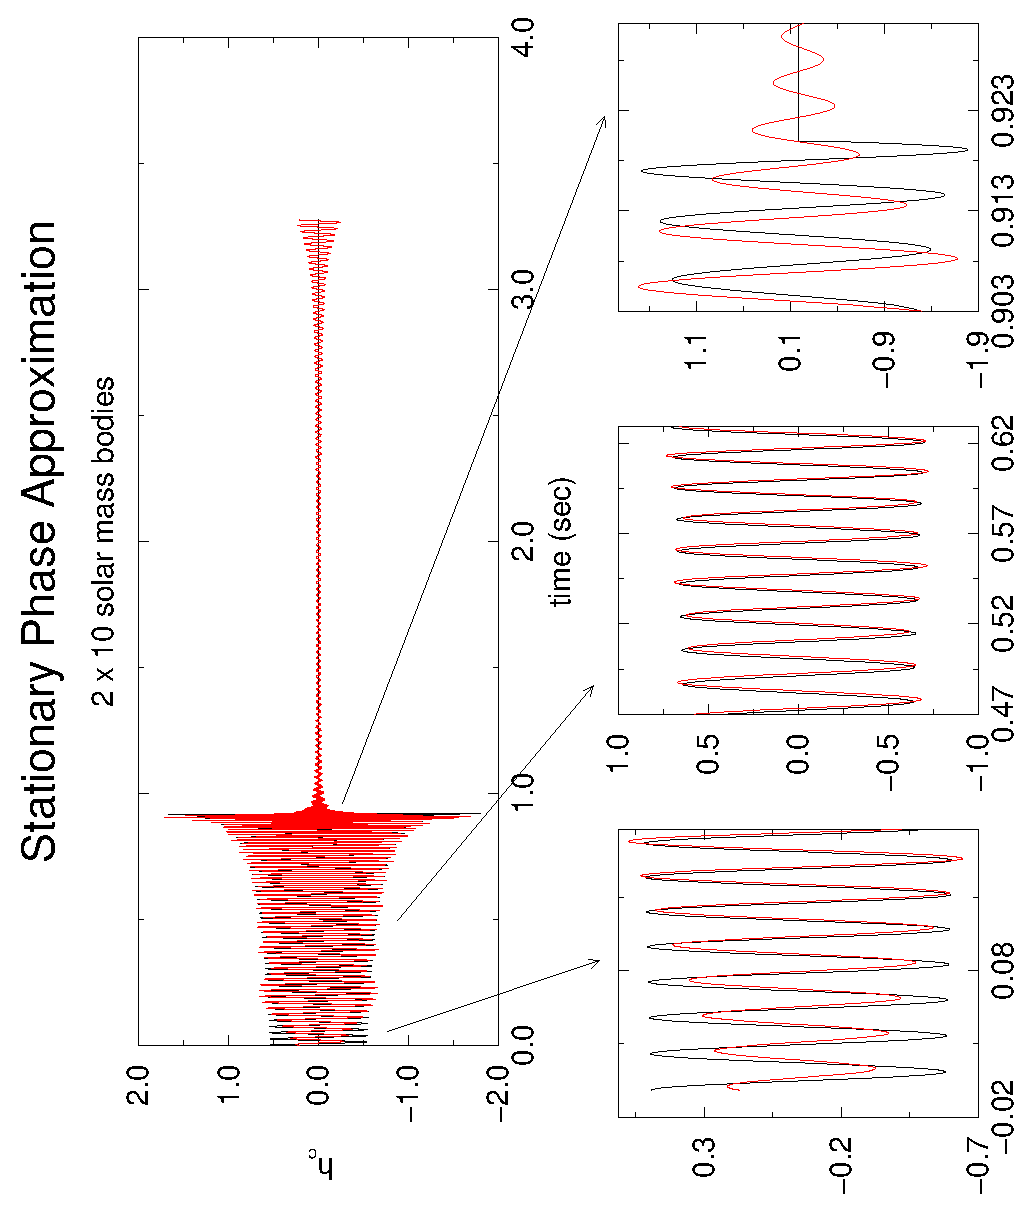
\epsfig{file=Figures/compare_chirps.ps,angle=-90,width=4.5in}
\caption{ \label{f:compare_chirps}
The output of {\tt compare\_chirps}, comparing the stationary-phase
approximate waveform FFT'd into the time domain (red curve) with a
2nd-order post-Newtonian chirp calculated in the time domain, using
{\tt make\_filters()} (black curve).  The lower part of the graph shows
three interesting regions of the upper (complete) graph.  The bottom
left detail shows the Gibbs startup-transient, the bottom middle detail
shows a typical region of good agreement, and the bottom right detail
shows the Gibbs turn-off transient.  The Gibbs startup transient is
also visible at the far right of the upper figure, which is
periodically identified with the far left.  }
\end{center}
\end{figure}



%%%%%%%%%%%%%%%%%%%%%%%%%%%%%%%%%%%%%%%%%%%%%%%%%%%%%%%%%%%%%%%%%%%%%%%%%%%%
%%%%%%%%%%%%%%%%%%    END OF BEN OWEN'S RESPONSIBILITY %%%%%%%%%%%%%%%%%%%%%
%%%%%%%%%%%%%%%%%%%%%%%%%%%%%%%%%%%%%%%%%%%%%%%%%%%%%%%%%%%%%%%%%%%%%%%%%%%%

\clearpage
\subsection{Wiener (optimal) filtering}
\label{ss:wienerfilt}
\setcounter{equation}0
The technique of {\it optimal filtering} is a well-studied and
well-understood technique which can be used to search for
characteristic signals (in our case, chirps) buried in detector noise.
In order to establish notation, we begin this section with a brief
review of the optimal filtering technique.

Suppose that the detector output is a dimensionless strain $h(t)$.  (In
Section~\ref{s:40meter} we show how to construct this quantity for the
CIT 40-meter prototype interferometer, using the recorded digital data
stream).  We denote by ${C}(t)$ the waveform of the signal (i.e.,
the chirp) which we hope to find, hidden in detector noise, in the
signal stream $h(t)$.  Since we would like to know about chirps which
start at different possible times $t_0$, we'll take ${C}(t) =
\alpha T(t-t_0)$ where $T(t)$ is the canonically normalized waveform 
of a chirp which enters the sensitivity band of the interferometer at 
time $t=0$. The constant $\alpha$ quantifies the strength of the signal
we wish to extract as compared to an otherwise identical signal of 
canonical strength (we will discuss how this canonical normalization
is defined shortly). In other words, $T(t)$ contains all the 
information about the chirp we are searching for apart from the 
arrival time and the strength, which are given by $t_0$ and $\alpha$ 
respectively. For the moment, we will ignore the fact that 
the chirps come in two different phase ``flavors".

We will construct a signal $S$, which is a number defined by
\begin{equation}
S = \int_{-\infty}^\infty dt \;h(t) Q(t),
\end{equation}
where $Q(t)$ is an optimal filter function in time domain, which we
will shortly determine in a way that maximizes the signal-to-noise
ratio $S/N$ or SNR.  We will assume that $Q$ is a real function of
time.

We use the Fourier transform conventions of (\ref{e:fft1}) and
(\ref{e:fft2}), in terms of which we can write the signal $S$ as
\begin{eqnarray}
\nonumber
S &=& \int_{-\infty}^\infty dt  \int_{-\infty}^\infty df  \int_{-\infty}^\infty df'
{\rm e}^{-2 \pi i f t+2 \pi i f' t} \tilde h(f) \tilde Q^* (f')\\
\nonumber
&=& 
\int_{-\infty}^\infty df  \int_{-\infty}^\infty df'
\delta(f-f') \tilde h(f) \tilde Q^* (f')\\
&=& 
\int_{-\infty}^\infty df \tilde h(f) \tilde Q^* (f).
\end{eqnarray}
This final expression gives the signal value $S$ written in the
frequency domain, rather than in the time domain.

Now we can ask about the expected value of $S$, which we denote 
$\langle S \rangle$. This is the average of $S$ over an ensemble of 
detector output streams, each one of which contains an identical 
chirp signal $C(t)$ but different realizations of the noise:
\begin{equation}
h(t) = C(t) + n(t).
\end{equation}
So for each different realization, $C(t)$ is exactly the same function,
but $n(t)$ varies from each realization to the next.  We will assume
that the noise has zero mean value, and that the phases are randomly
distributed, so that $\langle \tilde n(f) \rangle=0$.  We can then take
the expectation value of the signal in the frequency domain, obtaining
\begin{equation}
\langle S \rangle = \int_{-\infty}^\infty df \langle \tilde h(f)
\rangle \tilde Q^*(f) = \int_{-\infty}^\infty df \tilde C(f) \tilde
Q^*(f).
\end{equation}
We now define the {\it noise} $N$ to be the difference between the
signal value and its mean for any given element of the ensemble:
\begin{equation}
\label{e:noise}
N \equiv S-\langle S \rangle = \int_{-\infty}^\infty df \tilde n(f) \tilde Q^* (f).
\end{equation}
The expectation value of $N$ clearly vanishes by definition, so
$\langle N \rangle=0$.  The expected value of $N^2$ is non-zero,
however.   It may be calculated from the (one-sided) strain noise power
spectrum of the detector $S_h(f)$, which is defined by
\begin{equation}
\label{e:nspec}
\langle \tilde n(f) \tilde n^*(f') \rangle = {1 \over 2} S_h(|f|) \delta(f-f'),
\end{equation}
and has the property that 
\begin{equation}
\langle n^2(t) \rangle = \int_0^\infty S_h(f) \; df.
\end{equation}
We can now find the expected value of $N^2$, by squaring equation (\ref{e:noise}),
taking the expectation value, and using (\ref{e:nspec}), obtaining
\begin{eqnarray}
\nonumber
\langle N^2 \rangle &= & \int_{-\infty}^\infty df \int_{-\infty}^\infty
df' \tilde Q^*(f) \langle \tilde n(f)   \tilde n^*(f') \rangle \tilde
Q(f') \\
\nonumber
& = & {1 \over 2} \int_{-\infty}^\infty df \; S_h(|f|) |\tilde Q(f) |^2\\
\label{e:n2}
& = &  \int_{0}^\infty df \; S_h(f) |\tilde Q(f) |^2.
\end{eqnarray}
There is a nice way to write the formulae for the expected signal and
the expected noise-squared.  We introduce an ``inner product" defined
for any pair of (complex) functions $A(f)$ and $B(f)$.  The inner
product is a complex number denoted by $(A,B)$ and is defined by
\begin{equation}
\label{e:definprod}
(A,B) = \int_{-\infty}^\infty df \; {A(f) B^*(f) S_h(|f|)}.
\end{equation}
Because $S_h$ is positive, this inner product has the property that $(A,A)
\ge 0$ for all functions $A(f)$, vanishing if and only if $A=0$.  This
inner product is what a mathematician would call a ``positive definite
norm"; it has all the properties of an ordinary dot product of vectors
in three-dimensional Cartesian space.

In terms of this inner product, we can now write the expected signal, and the expected
noise-squared, as
\begin{equation}
\langle S \rangle = ({\tilde C \over S_h},\tilde Q)
\quad {\rm and} \quad \langle N^2 \rangle = {1 \over 2} (\tilde Q, \tilde Q).
\end{equation}
(Note that whenever $S_h$ appears inside the inner product, it refers
to the function $S_h(|f|)$ rather than $S_h(f)$.) Now the question is,
how do we choose the optimal filter function $Q$ so that the expected
signal is as large as possible, and the expected noise-squared is as
small as possible?  The answer is easy! Recall Schwarz's inequality for
inner products asserts that
\begin{equation}
        (A,B)^2 \le (A,A)(B,B),
\end{equation}
the two sides being equal if (and only if) $A$ is proportional to $B$.
So, to maximize the signal-to-noise ratio 
\begin{equation}
\label{e:sovern}
\left( {S \over N} \right)^2 ={\langle S \rangle^2 \over \langle N^2
\rangle} = 2 { ({\tilde C \over S_h},\tilde Q)^2 \over (\tilde Q,
\tilde Q)}
\end{equation}
we choose
\begin{equation}
\tilde Q(f) \propto {\tilde C(f) \over S_h(|f|)} = 
\alpha {\tilde T(f) \over S_h(|f|)} \; {\rm e}^{2 \pi i f t_0}.
\end{equation}
The signal-to-noise ratio defined by equation (\ref{e:sovern}) is normalized
in a way that is generally accepted and used.  Note that the definition is
independent of the normalization of the optimal filter $\tilde Q$, since
that quantity appears quadratically in both the numerator and denominator.
However if we wish to speak about ``Signal" values rather than about
signal-to-noise values, then the normalization of $\tilde Q$ is relevant.
If we choose the constant of proportionality to be $2 \alpha^{-1}$,
(i.e. set $\alpha = 2$, for reasons we will discuss shortly) then we
can express the template in terms of the canonical waveform,
\begin{equation}
\label{e:optimal}
        \tilde{Q}(f)=2 \> \frac{\tilde{T}(f)}{S_h(|f|)} {\rm e}^{2\pi i f t_0}
\end{equation}
Going back to the definition of our signal $S$, you will notice that the
signal $S$ for ``arrival time offset" $t_0$ is given by
\begin{eqnarray}
\nonumber
S &=& \int_{-\infty}^\infty df \; \tilde h(f) \tilde Q^* (f) \\
\label{e:lag}
  &=& 2 \int_{-\infty}^\infty df \; { \tilde h(f) \tilde T^* (f) 
\over S_h(|f|)} \; {\rm e}^{- 2 \pi i f t_0}.
\end{eqnarray}
Given a template $\tilde T$ and the signal $\tilde h$, the signal
values can be easily evaluated for any choice of arrival times $t_0$ by
means of a Fourier transform (or FFT, in numerical work).  Thus, it is
not really necessary to construct a different filter for each possible
arrival time; one can filter data for all possible choices of arrival
time with a single FFT.

The signal-to-noise ratio for this optimally-chosen filter can be
determined by substituting the optimal filter (\ref{e:optimal}) into
equation (\ref{e:sovern}), obtaining
\begin{equation}
\nonumber
\left( {S \over N} \right)^2 = 
 2 \int_{-\infty}^\infty df {| \tilde C(f) |^2 \over S_h(|f|)} =
 4 \int_{0}^\infty df { | \tilde C(f) |^2 \over S_h(f)} = 2 \alpha^2 
 \left(\frac{\tilde{T}}{S_h(|f|)},\frac{\tilde{T}}{S_h(|f|)}\right).
\end{equation}
You will notice that the signal-to-noise ratio $S/N$ in
(\ref{e:sovern}) is independent of the overall normalization of the
filter $Q$:  if we make $Q$ bigger by a factor of ten, both the
expected signal and the expected noise increase by exactly the same
amount.  For this reason, we can specify the normalization of the 
filter as we wish. Furthermore, it is obvious from (\ref{e:optimal}) 
that normalizing the optimal filter is equivalent to specifying the
normalization of the canonical signal waveform. It is traditional
(for example in Cutler and Flanagan \cite{cutler:1994})
to choose 
\begin{equation}
\label{e:cfnorm}
   \left(\frac{\tilde{T}}{S_h(|f|)},\frac{\tilde{T}}{S_h(|f|)}
   \right)=\frac{1}{2}.
\end{equation}
With this normalization, 
the expected value of the squared noise is
\begin{equation}
\langle N^2 \rangle = {1 \over 2} (\tilde Q,\tilde Q) = {1 \over 2} \>
\left( 2 \frac{\tilde{T}}{S_h(|f|)},2 \frac{\tilde{T}}{S_h(|f|)}
   \right) = 1
\end{equation}
and the signal-to-noise ratio takes the simple form
\begin{equation}
\left(\frac{S}{N}\right)^2 = \alpha^2.
\end{equation}
This adjustment or change of the filter normalization can be obtained 
by moving the (fictitious) astrophysical system emitting the chirp 
template either closer or farther away from us.  Because the metric 
strain $h$ falls off as $1/\rm distance$, the measured signal strength 
$S$ is then a direct measure of the inverse distance.

For example, consider a system composed of two  1.4 $M_\odot$ masses in
circular orbit.  Let us normalize the filter $\tilde T$ so that equation
(\ref{e:cfnorm}) is satisfied.  This normalization corresponds to placing
the binary system at some distance.  For the purpose of discussion,
suppose that this distance is 15 megaparsecs (i.e., choosing $T(t)$
to be the strain produced by an optimally-oriented two $\times$ 1.4
$M_\odot$ system at a distance of 15 megaparsecs).  If we then detect
a signal with a signal-to-noise ratio $S/N=30$, this corresponds to
detecting an optimally-oriented source at a distance of half a megaparsec.
Note that the normalization we have choosen has the r.m.s. noise $\sqrt{
\langle N^2 \rangle}= 1$ and therefore the signal and signal-to-noise
values are equal.

The functions {\tt correlate()} and {\tt productc()} are designed to
perform this type of optimal filtering.  We document these routines in
the following section and in Section~\ref{s:utility}, then provide a simple
example of an optimal filtering program.

There is an additional complication, arising from the fact that the
gravitational radiation from a binary inspiral event is a linear
combination of two possible orbital phases, as may be seen by reference
to equations (\ref{e:chirpcos}) and (\ref{e:chirpsin}).  Thus, the
strain produced in a detector is a linear combination of two waveforms,
corresponding to each of the two possible ($0^\circ$ and $90^\circ$)
orbital phases:
\begin{equation}
h(t) = \alpha T_{0}(t) + \beta T_{90}(t) + n(t).
\end{equation}
Here the subscripts $0$ and $90$ label the two possible orbital phases;
the constants $\alpha$ and $\beta$ depend upon the distance to the source
(and the normalization of the templates) and the orientation of the source
relative to the detector.  Thus $ T_{0}(t) $ denotes the (suitably
normalized) function $h_c(t)$ given by equation (\ref{e:chirpcos})
and $ T_{90}(t) $ denotes the (suitably normalized) function $h_s(t)$
given by equation (\ref{e:chirpsin}).

In the optimal filtering, we are now searching for a pair of amplitudes
$\alpha$ and $\beta$ rather than just a single amplitude.  One can easily do
this by choosing a filter function which corresponds to a complex-valued signal
in the time-domain:
\begin{equation}
\tilde Q(f) =   2 \>
{\tilde T_{0}(f) - i \tilde T_{90}(f) \over S_h(|f|)} \; {\rm e}^{2 \pi i f t_0}.
\end{equation}
We will assume that the individual filters for each polarization are
normalized by the convention just described, and that they are orthogonal:
\begin{equation}
\label{e:ono}
\left( {\tilde T_{0} \over S_h} , {\tilde T_{0} \over S_h} \right) = 
\frac{1}{2}, {\rm \ and\ }
\left( {\tilde T_{90} \over S_h} , {\tilde T_{90} \over S_h} \right) = 
\frac{1}{2}, {\rm \ and\ }
\left( {\tilde T_{0} \over S_h} , {\tilde T_{90} \over S_h} \right) = 0.
\end{equation}
Note that $T_{0}$ and $T_{90}$ are only exactly orthogonal in the
adiabatic limit where they each have many cycles in any frequency
interval $df$ in which the noise power spectrum $S_h(f)$ changes
significantly.  Also note that the filter function $\tilde Q(f)$ does
not correspond to a real filter $Q(t)$ in the time domain, since
$\tilde Q(-f) \ne \tilde Q^*(f)$, so that the signal
\begin{equation}
\label{e:complexsig}
S(t_0) = \left( {  \tilde h \over S_h}, \tilde Q \right)
\end{equation}
is a complex-valued functions of the lag $t_0$.  We define the noise as
before, by $N= S - \langle S \rangle$.  Its mean-squared modulus is
\begin{eqnarray}
\nonumber
\langle | N | ^2 \rangle &=& {1 \over 2} (\tilde Q,\tilde Q) \\
\nonumber
& = & 2 \left( {\tilde T_{0} -i \tilde T_{90} \over S_h} ,  
{\tilde T_{0} -i \tilde T_{90} \over S_h} \right) \\
& = & 2 \left[ \left( 
{\tilde T_{0} \over S_h} , {\tilde T_{0}  \over S_h} \right) +
\left( {\tilde T_{90}   \over S_h} , {\tilde T_{90}  \over S_h} \right) \right] = 2,
\end{eqnarray}
where we have made use of the orthornormality relation (\ref{e:ono}).
This value is twice as large as the expected noise-squared in the case of a single
phase waveform considered previously.

The expected signal at zero lag $t_0=0$ is
\begin{equation}
\langle S \rangle = \left( { \langle \tilde h \rangle \over S_h}, \tilde Q \right) =
2 \left( {\alpha \tilde T_{0}  + \beta \tilde T_{90} \over S_h} ,  
{\tilde T_{0} -i \tilde T_{90} \over S_h} \right) =  
\alpha +  i \beta.
\end{equation}
Hence the signal-to-noise ratio is
\begin{equation}
{\langle S \rangle \over \sqrt{\langle |N|^2 \rangle} } = \frac{1}{\sqrt{2}}
(\alpha + i \beta).
\end{equation}
In the absence of a signal $\langle S \rangle=0$ the expected value of the square of
this quantity (from the definition of $N$) is unity:
\begin{equation}
{\langle |S|^2 \rangle \over \langle |N|^2 \rangle} = 1.
\end{equation}
In the presence of a signal, the squared signal-to-noise ratio is
\begin{equation}
{| \langle S  \rangle |^2 \over \langle |N|^2 \rangle} = \frac{1}{2}
(\alpha^2 + \beta^2)
\end{equation}
In the case discussed previously, for a single-phase signal, we pointed out that
there was general agreement on the definition of signal-to-noise value.  In the present
case (a complex or two-phase signal) there is no such agreement.  The definition given
above is the one used by most experimenters: it is a quantity whose square has expected value
of unity in the absence of a signal.  However the definition often used in this
subject is
\begin{equation}
\left( {S \over N} \right)_{\rm Cutler\ and\ Flanagan} =
\left( {S \over N} \right)_{\rm Owen} =
\left( {S \over N} \right)_{\rm Thorne} = \max_{t_0} | S(t_0) |=
\sqrt{2} \left( {S \over N} \right)_{\rm GRASP}.
\end{equation}
Note that because ${S(t_0)}$ is complex, we maximize the modulus.
This is a quantity whose expected squared value, in the absence of a
signal, is 2.  To avoid confusion in the future, we will use a different
symbol for this quantity, and define
\begin{equation}
\rho \equiv 
\left( {S \over N} \right)_{\rm Cutler\ and\ Flanagan} =
\left( {S \over N} \right)_{\rm Owen} =
\left( {S \over N} \right)_{\rm Thorne} =
\sqrt{2} \left( {S \over N} \right)_{\rm GRASP}.
\end{equation}
This quantity is equal to the signal value alone (rather than the signal
value divided by the expected noise).

Another way to understand these two different choices of normalization,
and to understand why the conventional choice of normalization is $\rho$,
is that conventionally one treats the two-phase case in the same way
as the single phase case, but regards ${S \over N}$ as a function of a
phase parameter, $\theta = \arctan(\beta/\alpha)$.  For any fixed $\theta$,
${S \over N}(\theta)$ has rms value one, but the statistic $\max_\theta
{S \over N} (\theta)$ has rms value $\sqrt{2}$.

The attentive reader will notice, with our choice of filter and
signal normalizations, that we have lost a factor of $\sqrt{2}$ in the
signal-to-noise ratio compared to the case where we were searching for
only a single phase of waveform.  The expected signal strength in the
presence of a 0-phase signal is the same as in the single-phase case,
but the expected (noise)${}^2$ has been doubled.  This is because of the
additional uncertainty associated with our lack of information about the
relative contributions of the two orbital phases.  In other words, if we
know in advance that a waveform is composed entirely of the zero-degree
orbital phase, then the expectation value of the signal-to-noise,
determined by equation (\ref{e:sovern}) would be given by $\langle S
\rangle/N = \sqrt{2} \alpha$.  However if we need to search for the
correct linear combination of the two possible phase waveforms, then
the expectation value of the signal-to-noise is reduced to  $\langle
S \rangle/N = \alpha$.  However, as we will see in the next section,
this reduction in signal-to-noise ratio does not significantly affect
our ability to detect signals with a given false alarm rate.
\clearpage

\subsection{Comparison of signal detectability for single-phase and two-phase searches}
\label{ss:compare12}
The previous Section \ref{ss:wienerfilt} described optimal filtering searches in two cases -
looking for:
\begin{itemize}
\item 
A signal of known phase, proportional to $T_0$, and
\item
A signal of unknown phase, which is some linear
combinations of $T_0$ and $T_{90}$.
\end{itemize}
With the choice of filter normalizations made previously, the expected
signal produced by a source $\alpha T_0$ would be the same for both
searches, but the expected (noise)${}^2$ was higher in the two-phase case.
One might wonder if this reduced SNR means that a two-phase search reduces
ones ability to identify signals.  The answer turns out to be ``not significantly".

The reason for this is that the distribution of signal values produced
by detector noise alone in the single- and two-phase cases are quite
different.  In order to answer the question: ``what is the smallest
signal detectable" we need to fix a false alarm rate.  For a given
time-duration of data, this is equivalent to fixing a false alarm
probability.  Let us assume that this probability has been fixed to be
a small value $\epsilon$, and compare the single- and two-phase searches.

In the single-phase case, in the absence of a source, the values of
the signal $S$ (\ref{e:lag}) are Gaussian random variables with a
mean-squared value of 1.  Hence the threshold $S_0$ determined by the
false alarm rate must be set so that there is probability $\epsilon$
of $S$ falling outside the range $[-S_0,S_0]$.  This means that
\begin{equation} \epsilon = 2 {1 \over
\sqrt{2 \pi}} \int_{S_0}^\infty \exp(-x^2/2) \> dx = {\rm \ erfc} (S_0/\sqrt{2}) .
\end{equation}
The solution to this equation is the threshold as a function of the false alarm
probability:
\begin{equation}
S_0^{\small \textrm{single-phase}}(\epsilon)=\sqrt{2}
{\rm \ erfc}^{-1}(\epsilon).
\end{equation}
Thus, for example, to obtain a false alarm probability of $\epsilon =
10^{-5}$ we need to set a threshold $S^{\small \textrm{single-phase}}_0
= \sqrt{2} \textrm{\ erfc}^{-1}(10^{-5}) = 4.417$.  In this case, our
minimum detectable signal has amplitude $\alpha = 4.417$.

In the two-phase case, the probability distribution of the signal in
the absence of a source is different, because in this case the signal
(\ref{e:complexsig}) is described by the probability distribution of
a random variable $r$, where $r^2 = x^2 + y^2$ and $x$ and $y$ are
independent random Gaussian variables with unit rms.   Here, $x$ and
$y$ are the real and imaginary parts of the signal (\ref{e:complexsig}
in the absence of a source.  Their probability distribution is:
\begin{eqnarray}
\nonumber
P(x) dx P(y) dy & = & {1 \over 2 \pi} {\rm e}^{-x^2/2} {\rm e}^{-y^2/2} dx dy \\
                & = & {1 \over 2 \pi} {\rm e}^{-r^2/2} r dr d\phi \\
\nonumber
   & \Rightarrow  &\\
   P(r)dr & = &  {\rm e}^{-r^2/2} r dr.
\end{eqnarray}
In the final line, we have integrated over the irrelevant angular variable
$\phi \in [0,2\pi)$.  So in the two-phase case, as before, the threshold value of the
signal is set by requiring that the false alarm probability be $\epsilon$:
\begin{equation}
\epsilon=\int_{S_0}^\infty \exp(-r^2/2) r dr = \exp({-S_0^2/2}).
\end{equation}
The solution here is that the threshold is
$S^{\small \textrm{two-phase}}_0 = \sqrt{-2  \ln
\epsilon}$.  For example, to obtain a false alarm probability of $\epsilon
= 10^{-5}$ we need to set a threshold $S^{\small \textrm{two-phase}}_0 = 4.799$.  In this case,
our minimum detectable (0-phase) signal has amplitude $\alpha = 4.799$,
which is only slightly higher than in the single-phase case.

It is not a coincidence that for a given false alarm rate, the amplitude
of the minimum detectable signals are almost the same.  Although the
expected value of the single-phase signal${}^2$ in the absence of a source
is smaller than the expected value of the two-phase $|{\rm signal}|^2$
in the absence of a source, the {\it tails} of the two probability
distributions are almost identical.  For the same false alarm probability
$\epsilon$ the thresholds in the two instances are related by
\begin{equation}
\epsilon=
\sqrt{2 \over \pi} \int_{S^{\small \textrm{single-phase}}_0}^\infty \exp(-x^2/2) \>dx
=
\int_{S^{\small \textrm{two-phase}}_0}^\infty \exp(-r^2/2) r dr
\end{equation}
But for thresholds of reasonable size (small $\epsilon$) both integrals
are dominated by the region just to the right of $S_0$, and in this neighborhood the
integrands differ by a small factor of approximately $\sqrt{\pi S_0 \over 2}$.
Since $\epsilon$ varies exponentially with the threshold, there is a logarithmically
small difference between the thresholds $S^{\small \textrm{single-phase}}_0$ and
$S^{\small \textrm{two-phase}}_0$.

For a fixed false alarm probability, we can write the the two-phase
threshold $S^{\small \textrm{two-phase}}_0$ as a function of the
one-phase threshold $S^{\small \textrm{single-phase}}_0$:
\begin{equation}
S^{\small \textrm{two-phase}}_0 = \sqrt{ - 2 \ln \left(\textrm{erfc}\left({S^{\small \textrm{single-phase}}_0 \over \sqrt{2}}\right) \right)}.
\end{equation}
The plot of this relationship in Figure \ref{f:thresholds} shows clearly
that once the thresholds are reasonably large, they are very nearly equal.
\begin{figure}[h]
\begin{center}
\epsfig{file=Figures/thresholds.ps,angle=0,width=3.5in}
\caption{ \label{f:thresholds} The threshold for a two-phase search
$S^{\small \textrm{two-phase}}_0$ is shown as a function of the threshold
for the single-phase search $S^{\small \textrm{single-phase}}_0$ which
gives the same false alarm rate.  When the false alarm rates are small,
they are very nearly equal.  }
\end{center}
\end{figure}

\clearpage

\subsection{Function: \tt correlate()}
\label{ss:correlate}
\setcounter{equation}0
{\tt void correlate(float *s,float *h,float *c,float *r,int n)}\\
This function evaluates the correlation (as a function of lag time $t$)
defined by the discrete equivalent of equation (\ref{e:lag}):
\begin{equation}
\label{e:corrdef}
s(t) = {1 \over 2} \int_{-\infty}^\infty df \; { \tilde h(f) \tilde c^* (f) \tilde r (f) }
 \; {\rm e}^{- 2 \pi i f t}.
\end{equation}
It is assumed that $\tilde h(f)$ and $\tilde c(f)$ are Fourier
transforms of real functions, and that $\tilde r(f)$ is real.  The factor of
$1/2$ appears in (\ref{e:corrdef}) for efficiency reasons; in order to calculate
the integral (\ref{e:lag}) one should set $\tilde r(f) = 2/S_h(f)$.  The routine
assumes that $\tilde r$ vanishes at both DC and the Nyquist frequency.

The arguments are:
\begin{description}
\item{\tt s}: Output.  Upon return, the array {\tt s[0..n-1]} contains
  the correlation $s(t)$ at times 
  \begin{equation}
   \nonumber
    t=0,\Delta t, 2 \Delta t,\cdots,(n-1) \Delta t.
  \end{equation}
\item{\tt h}: Input.  The array {\tt h[0..n-1]} contains the positive
  frequency ($f \ge 0$) part of the complex function $\tilde h(f)$.
  The packing of $\tilde h$ into this array follows the scheme used by
  the {\it Numerical Recipes} routine {\tt realft()}, which is
  described between equations (12.3.5) and (12.3.6) of \cite{NumRec}.
  The DC component $\tilde h(0)$ is real, and located in {\tt h[0]}.
  The Nyquist-frequency component $\tilde h(f_{\rm Nyquist})$ is also
  real, and is located in {\tt h[1]}.  The array elements {\tt h[2]}
  and {\tt h[3]} contain the real and imaginary parts, respectively, of
  $\tilde h(\Delta f)$ where $\Delta f = 2 f_{\rm Nyquist}/n = (n
  \Delta t)^{-1}$.   Array elements {\tt h[2j]} and {\tt h[2j+1]}
  contain the real and imaginary parts of $\tilde h( j \; \Delta f)$
  for $j=1,\cdots,n/2-1$.  It is assumed that $\tilde h(f)$ is the
  Fourier transform of a real function, so that {\tt correlate()} can
  infer the negative frequency components from the equation $\tilde
  h(-f) = \tilde h^*(f)$
\item{\tt c}: Input.  The array {\tt c[0..n-1]} contains the complex
  function $\tilde c$, packed in the same format as $\tilde h(f)$,
  with the same assumption that $\tilde c(-f) = \tilde c^*(f)$.
  Note that while you provide the function $\tilde c(f)$ to the
  routine, it is the {\it complex-conjugate} of the function contained
  in the array {\tt c[ ]} which is used in calculating the correlation.
  Thus if $\tilde r$ is positive, {\tt correlate(s,c,c,r,n)} will
  always return ${\tt s[0]}\ge 0$.
\item{\tt r}: Input.  The array {\tt r[0..n/2]} contains the values of
  the real function $\tilde r$ used as a weight in the integral.  This
  is often chosen to be (twice!) the inverse of the receiver noise, as
  in equation (\ref{e:lag}), so that $\tilde r(f) = 2/\tilde
  S_h(|f|)$.  The array elements are arranged in order of increasing
  frequency, from the DC value at subscript 0, to the Nyquist frequency
  at subscript n/2.  Thus, the $j$'th array element {\tt r[j]} contains
  the real value $\tilde r(j \; \Delta f)$, for $j=0,1,\cdots,n/2$.
  Again it is assumed that $\tilde r(-f) = \tilde r^*(f) = \tilde r(f)$.
\item{\tt n}: Input.  The total length of the complex arrays
  {\tt h} and {\tt c}, and the number of points in the output
  array {\tt s}.  Note that the array {\tt r} contains $n/2+1$
  points.  n must be even.
\end{description}
The correlation function calculated by this routine is ${1 \over 2} FFT^{-1}[\tilde
h \tilde c^* \tilde r]$ and has the same dimensions as the product
$\tilde h \times \tilde c \times \tilde r$.  The definition is
\begin{equation}
{\tt s}_k = {1 \over 2} \sum_{j=0}^{{\tt n}-1} {\tt h}_j {\tt c}^*_j {\tt r}_j
{\rm e}^{- 2 \pi i j k/{\tt n}}
\end{equation}
where it is understood that ${\tilde h}_{{\tt n}-j} = \tilde h^*_j$ and
that ${\tilde c}_{{\tt n}-j} = \tilde c^*_j$, and that
${\tilde r}_{{\tt n}-j} = \tilde r_j$. 

Note that the input arrays
{\tt h[ ]} and {\tt c[ ]} can be the same array.  For example {\tt
correlate(s,c,c,r,n)} calculates the discrete equivalent of
\begin{equation}
s(t) = {1 \over 2} \int_{-\infty}^\infty df \; { |\tilde c (f) |^2 \tilde r (f) }
 \; {\rm e}^{- 2 \pi i f t}.
\end{equation}

\begin{description}
\item{Author:}
Bruce Allen, ballen@dirac.phys.uwm.edu
\item{Comments:}
For the sake of efficiency, this function does not include the
contribution from either DC or Nyquist frequency bins to the
correlation (these are negligible in any sensible data).
\end{description}
\clearpage

\subsection{Function: {\tt avg\_inv\_spec()}}
\label{ss:avg_inv_spec}
\setcounter{equation}0
{\tt  void avg\_inv\_spec(float flo,float srate,int n,double decay,double *norm,
                  float *htilde, float* mean\_pow\_spec,float* twice\_inv\_noise)}\\
This function maintains an auto-regressive moving average (see {\tt
avg\_spec()}) of the power spectrum $S_h(f)$, and an array containing
$2/S_h(f)$, which can be used for optimal filtering.  This latter array
is set to zero below a specified cuff-off frequency $f_{low}$.

The arguments are:
\begin{description}
\item{\tt flo:} Input.  The low frequency cut-off $f_{low}$, in Hz.
\item{\tt srate:} Input.  The sample rate, in Hz.
\item{\tt n:} Input.  The number of points in the arrays.
\item{\tt decay:} Input.  The quantity $\exp(-\alpha)$ as defined in {\tt avg\_spec()}.
  Sets the characteristic decay time for the auto-regressive average.
\item{\tt norm:} Input/Ouput.  Used for internal storage.  Set to $0$ when you want to begin
   a new auto-regressive average.  Must not be altered otherwise.
\item{\tt htilde:} Input.  The array {\tt htilde[0..n-1]} contains the positive frequency FFT of
   the metric perturbation.
\item{\tt mean\_pow\_spec:} Output.  The array {\tt mean\_pow\_spec[0..n/2]} contains the 
  mean power spectrum.  Should be zeroed when resetting to begin a new average.  The array
element {\tt mean\_pow\_spec[0]} contains the power spectrum at DC, and the array
element {\tt mean\_pow\_spec[n/2]} contains the power spectrum at the Nyquist frequency
{\tt srate}/2.
\item{\tt twice\_inv\_noise:} Output.  The array {\tt
   twice\_inv\_noise[0..n/2]} contains $2/S_h(f)$.  It is set to zero for
   $f<f_{low}$.  The array element {\tt twice\_inv\_noise[0]} contains
   the DC value, and the array element {\tt twice\_inv\_noise[n/2]}
   contains the value at the Nyquist frequency {\tt srate}/2.
\end{description}
\begin{description}
\item{Author:}
Bruce Allen, ballen@dirac.phys.uwm.edu
\item{Comments:}
We assume here that the ``correct" thing to do is the average the
spectrum, then invert it.  There may be a better way to construct
the weight function for an optimal filter, however.
\end{description}
\clearpage

\subsection{Function: {\tt orthonormalize()}}
\label{ss:orthonormalize}
\setcounter{equation}0
{\tt void orthonormalize(float* ch0tilde, float* ch90tilde, float* twice\_inv\_noise, int n, float* n0, float* n90)}\\
This function takes as input the (positive frequency parts of the) FFT
of a pair of chirp signals.  Upon return, the $90^\circ$ phase chirp
has been made orthogonal to the $0^\circ$ phase chirp, with respect to
the inner product defined by $2/S_h$.  The normalizations of the chirps
are also returned.

The arguments are:
\begin{description}
\item{\tt ch0tilde:} Input.  The FFT of the zero-phase chirp $T_0$.
\item{\tt ch90tilde:} Input/Output.  The FFT of the $90^\circ$-phase chirp $T_{90}$.
\item{\tt twice\_inv\_noise:} Input.  Array containing $2/S_h$.
The array element {\tt twice\_inv\_noise[0]} contains
   the DC value, and the array element {\tt twice\_inv\_noise[n/2]}
   contains the value at the Nyquist frequency.
\item{\tt n:} Input. Defines the length of the arrays: {\tt ch0tilde[0..n-1]}, {\tt ch90tilde[0..n-1]},
  and {\tt twice\_inv\_noise[0..n/2]}.
\item{\tt n0:} Output.  The normalization of the 0-phase chirp.
\item{\tt n90:} Output.  The normalization of the $90^\circ$-phase chirp.
\end{description}

Using the notation of (\ref{e:definprod}) one may define an inner product of the
chirps.  The normalizations are defined as follows:
\begin{equation}
{1 \over n_0^2} \equiv {1 \over 2} (Q_0,Q_0),
\end{equation}
where $Q_0$ is the optimal filter defined for the zero-phase chirp $T_0$.
The chirps are orthogalized internally using the Gram-Schmidt procedure.
We first calculate $(Q_0,Q_0)$ and $(Q_{90},Q_{0})$ then define
$\epsilon = (Q_{90},Q_{0})/(Q_0,Q_0)$.  We then modify the $90^\circ$-phase chirp
setting
$\tilde T_{90} \rightarrow T_{90} - \epsilon T_0$.  This ensures that the
inner product $(Q_{90},Q_{0})$ vanishes.  The normalization for this newly-defined
chirp is then defined by
\begin{equation}
{1 \over n_1^2} \equiv {1 \over 2} (Q_{90},Q_{90}).
\end{equation}
\begin{description}
\item{Author:}
Bruce Allen, ballen@dirac.phys.uwm.edu
\item{Comments:}
Notice that the filters $Q_0$ and $Q_{90}$ are not in general
orthogonal except in the adiabatic limit as $S_h(f)$ varies very slowly
with changing $f$.  Our approach to this is to construct a
slightly-modified ninety-degree phase signal.  Note however that this
may introduce small errors in the determination of the orbital phase.
This should be quantified.
\end{description}
\clearpage


\subsection{Dirty details of optimal filtering: wraparound and windowing}
\label{ss:dirty}
To carry out optimal filtering, we need to break the data set (which
might be hour, days, or weeks in length) into shorter stretches of $N$
points (which might be seconds or minutes in length). We can understand
the effects of ``chopping up" the data most easily in the case for
which (1) the instrument noise is {\it white}, so that $S_h(f)=1$; (2)
the source is so close that its signal overwhelms the noise in the
IFO, and (3) we are looking for a signal with a given phase (not a
linear combination of the two orbital phases).

We want to calculate a signal $S$ as a function of lag $t_0$ using
an FFT.
\begin{equation}
S(t_0) = \int h(t) T(t-t_0) dt \approx
S(i_0) = \sum_j h_j T_{j-i_0},
\end{equation}
where we have written both the continuous-time and discrete-time version
of the same equation.  Using the definition of the discrete Fourier
transform, and writing
\begin{equation}
h_j = \sum_{k=0}^{N-1} {\rm e}^{-2 \pi i j k/N} \tilde h_k \quad
{\rm and } \quad
T_{j-i_0} = \sum_{k'=0}^{N-1} {\rm e}^{-2 \pi i (j-i_0) k'/N} \tilde T_{k'} \quad
\end{equation}
one can easily compute that the signal as a function of lag $i_0$
is
\begin{eqnarray}
S(i_0) &=& \sum_{j=0}^{N-1} \sum_{k=0}^{N-1} \sum_{k'=0}^{N-1}
{\rm e}^{-2 \pi i j k/N} \tilde h_k 
{\rm e}^{-2 \pi i (j-i_0) k'/N} \tilde T_{k'} \\ 
&=& \sum_{k=0}^{N-1} \sum_{k'=0}^{N-1} N \delta_{k,-k'} 
{\rm e}^{2 \pi i i_0 k'/N} \tilde h_k \tilde T_{k'} \\
&=& \sum_{k=0}^{N-1}   N   
{\rm e}^{-2 \pi i i_0 k/N} \tilde h_k \tilde T^*_{k}.
\end{eqnarray}
Thus, if the data is treated as periodic, and the template is treated as
periodic, one can compute the correlation as a function of time using only
an FFT.  In particular, the use of rectangular windowing does create
sidelobes of the template's frequency components.  However it also creates
identical sidelobes of the signal's frequency components - so in effect the
correlation in the time domain can be calculated exactly, without any windowing
of the signal being necessary.

The only complication arises from the fact that the FFT treats the data
as being periodic.  Let's consider some simple examples to illustrate
the effects of this.   In all of our examples, the number of data
points is $N=65,536=2^{16}$ and the (schematic) chirp filter has length
$m=13,500$ and is zero-padded after that time.   Please remember, in
all the figures that follow, to identify the far right hand side of the
graph ($i=65535$) with the far left hand side ($i=0$).
Figure~\ref{f:chirpa} shows $S(i_0)$ for a schematic chirp which begins
at the first data point in the rectangular window.  You will notice
that the filter output peaks at $i=0$.
\begin{figure}[h]
\index{colorpage}
\begin{center}
\epsfig{file=Figures/fig12a.ps,angle=-90,width=4.5in}
\caption{ \label{f:chirpa} A chirp starting at initial time $i=0$ and
ending at time $i=13500$ is processed through a chirp filter, whose
output peaks at time $i=0$.  Notice that because of wraparound, the
(non-causal) filter output begins ``earlier" than $i=0$.}
\end{center}
\end{figure}
If the incoming chirp arrives somewhat later (it starts at $i=15,000$)
as shown in Figure~\ref{f:chirpb} then the filter output peaks at the
start time, as shown.
\begin{figure}[h]
\index{colorpage}
\begin{center}
\epsfig{file=Figures/fig12b.ps,angle=-90,width=4.5in}
\caption{ \label{f:chirpb} A chirp starting at initial time $i=15,000$ and
ending at time $i=28,500$ is processed through a chirp filter, whose
output peaks at time $i=15,000$.}
\end{center}
\end{figure}
A chirp in the signal which starts at the $i=65,535-13,500$ as shown in
Figure~\ref{f:chirpc} causes the filter output to peak at $i=52,035$.
\begin{figure}[h]
\begin{center}
\epsfig{file=Figures/fig12c.ps,angle=-90,width=4.5in}
\index{colorpage}
\caption{ \label{f:chirpc} A chirp starting at initial time $i=52,035$.}
\end{center}
\end{figure}
Thus, in order to find chirps, we need to find the maxima of the filter
output over the interval $i=0\cdots,N-m$.

Chirp filters can be ``stimulated" or ``triggered" by events that are
not chirps.  We will shortly discuss some techniques that can be used
to distinguish triggering events that are chirps from those that are
simply noise spikes or other transient (but non-chirp) varieties of
non-stationary interferometer noise.  Suppose that a chirp filter is
triggered by some kind of transient event in the IFO output.  At what
time did this transient event ocurr?  The answer to this question can
be seen by examining the impulse response of the ``periodic filter"
scheme, as shown in the following figures.
\begin{figure}[h]
\begin{center}
\epsfig{file=Figures/fig12d.ps,angle=-90,width=4.5in}
\index{colorpage}
\caption{ \label{f:chirpd} An impulse shortly after $i=0$.}
\end{center}
\end{figure}
\begin{figure}[h]
\begin{center}
\epsfig{file=Figures/fig12e.ps,angle=-90,width=4.5in}
\index{colorpage}
\caption{ \label{f:chirpe} An impulse at $i=15,000$.}
\end{center}
\end{figure}
\begin{figure}[h]
\begin{center}
\index{colorpage}
\epsfig{file=Figures/fig12f.ps,angle=-90,width=4.5in}
\caption{ \label{f:chirpf} An impulse at $i=28,500$.}
\end{center}
\end{figure}
\begin{figure}[h]
\begin{center}
\epsfig{file=Figures/fig12g.ps,angle=-90,width=4.5in}
\index{colorpage}
\caption{ \label{f:chirpg} An impulse shortly before $i=65535$}
\end{center}
\end{figure}
Thus, by searching for maxima in the filter output over the range
$i=0,\cdots,N-m-1$ we can detect either true chirps in the data stream,
starting in the time interval $i=0,\cdots,N-m-1$ and coalescing
(roughly speaking) in the time interval $i=m,\cdots, N-1$, or we can
detect transient impulse-like events in the data stream, which take
place in the time interval $i=m,\cdots, N-1$.  In the GRASP optimal
filtering code, after examining the stretch of $N$ data points, we then
shift the data points $i=N-m,\cdots,N-1$ into the range
$i=0,\cdots,m-1$ and acquire a new additional set of $N-m$ data points
covering remaining (new) time interval.

To indicate the time at which the filter output reached its maximum,
several different conventions can be used.  First, we can indicate the
{\it peak offset}.  This is the offset from the start of the filter output
at which the filter output reaches a maximum value.  Alternatively,
we can use the {\it impulse offset}.  This is the
offset at which the filter would have peaked if the maximum were due
to a delta-function like impulse at the input. These quantities
are defined in equation (\ref{e:impulsevspeak}).

Note that in practice, because the chirp signal has to be convolved
with the response function $R(f)$ of the detector, the impulse response
of the filter is typically a few points longer than the actual chirp
signal.  For this reason it is smart to assume that the impulse
response of your optimal filter is slightly longer (say a hundred
points longer) than the actual time-domain length of the corresponding
chirp.  This safety margin is set with the
{\tt {\#d}efine SAFETY} statement in the optimal filtering example.
You lose a tiny bit of efficiency but reduce the likelihood
that boundary effects from the data discontinuity at the start/end of
the rectangular window will significantly stimulate the optimal filter
output for $i=0,\cdots,N-m-1$. (See Figs.~\ref{f:chirpd} and
\ref{f:chirpg} to see an illustration of how this windowing
discontinuity will corrupt the filter's output.)

We have demonstrated explicitly that with no windowing (or rather,
rectangular windowing) of the data, one can find the appropriate
correlation between the signal and a filter exactly: the rectangular
window has the same effect on the signal as it does on the template
(shifting energy into sidelobes in identical fashion).  The only
complication was that because of the periodic nature of the FFT one has
to be caseful about wrap-around errors in relating the output of a
filter to the time of occurrence of a signal or impulse.

There is one remaining ugly question.  The optimal filter $\tilde Q$
depends upon the noise power spectrum of the detector.  In real-world
filtering, should this noise power spectrum be calculated with
windowed, or non-windowed data?  We can determine the correlation
between signal and template exactly, with only rectangular windowing,
because energy in either of these functions is shifted into sidelobes
in identical fashion.  However a ``quiet" part of the IFO spectrum can
be corrupted by sidelobes of a nearby noisy region.  The effect of this
is that the signal get rather less weight from this region of frequency
space than it ought, in theory, to receive.  This would argue for using
only properly-windowed data to find the noise power spectrum to use in
determining an optimal filter.

In fact, in our experience, it does not make any difference, at least
not when you are searching for binary inspiral chirps.  The reason is
that the SNR obtained in an optimal filter is only sensitive at second
order to errors in the optimal filter function.  Thus, the errors due
to noise sidelobes which appear if you fail to window the data to
calculate an optimal filter are typically not large.
\clearpage


\subsection{Function: {\tt find\_chirp()}}
\label{ss:find_chirp}
\setcounter{equation}0
{\tt void find\_chirp(float* htilde, float* ch0tilde, float* ch90tilde, float* twice\_inv\_noise, float n0, float n90, 
                float* output0, float* output90, int n, int chirplen, int*
                offset, float* snr\_max, float* c0, float* c90, float
                *var) }\\
This routine filters the gravity-wave strain through a pair of optimal
filters corresponding to the two phases of a binary chirp, then finds
the time at which the SNR peaks.

The arguments are:
\begin{description}
\item{\tt htilde}: Input.  The FFT of the gravity-wave strain.
\item{\tt ch0tilde}: Input.  The FFT of the 0-degree chirp.
\item{\tt ch90tilde}: Input.  The FFT of the 90-degree chirp (assumed orthogonal to the 0-degree chirp).
\item{\tt twice\_inv\_noise}: Input.  Twice the inverse noise power spectrum, used for optimal filtering.
The array element {\tt twice\_inv\_noise[0]} contains
   the DC value, and the array element {\tt twice\_inv\_noise[n/2]}
   contains the value at the Nyquist frequency.
\item{\tt n0:} Input.  Normalization of the 0-degree chirp.  
\item{\tt n90:} Input.  Normalization of the 90-degree chirp.
\item{\tt output0:} Output.  A storage array.  Upon return, contains the filter output of the 0-degree
  phase optimal filter.
\item{\tt output90:} Output.  A storage array.  Upon return, contains the filter output of the 90-degree
  phase optimal filter.
\item{\tt n:} Input.  Defines the lengths of the various arrays: {\tt
  ch0tilde[0..n-1]}, {\tt ch90tilde[0..n-1]}, {\tt output0[0..n-1]},
  {\tt output90[0..n-1]}, and {\tt twice\_inv\_noise[0..n/2]}.
\item{\tt chirplen:} Input.  The number of bins in the time domain occupied by the chirp that you
   are searching for.  This is necessary in order to untangle the wrap-around ambiguity explained earlier.
\item{\tt offset:} Output.  The offset, from 0 to {\tt n-chirplen-1},
  at which the signal output (for an arbitrary linear combination of the two filters) peaks.
\item{\tt snr\_max:} Output.  The maximum signal-to-noise ratio (SNR) found.
\item{\tt c0:} Output.  The coefficient of the 0-phase template which achieved the highest SNR.
\item{\tt c90:} Output.  The coefficient of the $90^\circ$-phase
  template which achieved the highest SNR.  Note that $c_0^2 + c_{90}^2$ should be 1.
\item{\tt var:} Output.  The variance of the filter output.  Would be 1 if the input to
   the filter were colored Gaussian noise with a spectrum defined by $S_h$.
\end{description}
\begin{description}
\item{Author:}
Bruce Allen, ballen@dirac.phys.uwm.edu
\item{Comments:}
None.
\end{description}
\clearpage

\subsection{Function: {\tt freq\_inject\_chirp()}}
\label{ss:freq_inject_chirp}
\setcounter{equation}0
{\tt void freq\_inject\_chirp(float c0, float c90, int offset, float
    invMpc, float* ch0tilde, float* ch90tilde, float* htilde, int n) }\\
The bottom-line test of any optimal filtering code or searching
routines is: can you inject ``fake" signals into the data stream, and
properly detecting them, while properly rejecting all other signatures
of instrumental effects, etc.  This routine injects artificial signals
into the frequency-domain strain $\tilde h(f)$.  The plane of the binary
system is assumed to be normal to the line to the detector.

The arguments are:
\begin{description}
\item{\tt c0:} Input. The coefficient of the 0-phase template to inject.
\item{\tt c90:} Input. The coefficient of the $90^\circ$-phase to
   inject.  Note that $c_0^2 + c_{90}^2$ should be 1.
\item{\tt offset:} Input. The offset number of samples at which the injected chirp starts, in the
   time domain.
\item{\tt invMpc:} Input. The inverse of the distance to the system
(measured in Mpc).
\item{\tt ch0tilde:} Input. The FFT of the phase-0 chirp (strain units)
at a distance of 1 Mpc.
\item{\tt ch90tilde:} Input. The FFT of the phase-90 chirp (strain units)
at a distance of 1 Mpc.
\item{\tt htilde:} Output. The FFT of the gravity-wave strain.  Note that
this routine {\it adds into} and increments this array, so that if it
contains another ``signal" like IFO noise, the chirp is simply super-posed
onto it.
\item{\tt n:} Input.  Defines the lengths of the various arrays {\tt ch0tilde[0..n-1]},
{\tt ch90tilde[0..n-1]}, and {\tt htilde[0..n-1]}.
\end{description}

Note that in making use of this injection routine, you must determine
the level of the quantization noise of the ADC, and be careful to
inject a properly dithered version of this signal when its amplitude
is small compared to the ADC quantization step size.

\begin{description}
\item{Author:}
Bruce Allen, ballen@dirac.phys.uwm.edu
\item{Comments:}
See the comments for {\tt time\_inject\_chirp}, particularly with respect to
the digital quantization noise.
\end{description}
\clearpage

\subsection{Function: {\tt time\_inject\_chirp()}}
\label{ss:time_inject_chirp}
\setcounter{equation}0
{\tt void time\_inject\_chirp(float c0, float c90, int offset, float
    invMpc, float* chirp0, float* chirp90, float* data, float *response, float *work, int n) }\\
This is a time-domain version of the previous function {\tt
freq\_inject\_chirp()} which injects chirps in the time-domain (after
deconvolving them with the detector's response function).  This routine
injects artificial signals into the time-domain strain $h(t)$.  The
plane of the binary system is assumed to be normal to the line to the
detector.

The arguments are:
\begin{description}
\item{\tt c0:} Input. The coefficient of the 0-phase template to inject.
\item{\tt c90:} Input. The coefficient of the $90^\circ$-phase to
   inject.  Note that $c_0^2 + c_{90}^2$ should be 1.
\item{\tt offset:} Input. The offset number of samples at which the injected chirp starts, in the
   time domain.
\item{\tt invMpc:} Input. The inverse of the distance to the system (measured in Mpc).
\item{\tt chirp0:} Input. The time-domain phase-0 chirp (strain units) at a distance of 1 Mpc.
\item{\tt chirp90:} Input. The time-domain phase-90 chirp (strain units) at a distance of 1 Mpc.
\item{\tt data:} Output. The detector response in time that would be produced by the
 specified binary inspiral.  Note that this routine {\it adds into} and
 increments this array, so that if it contains another ``signal" like
 IFO noise, the chirp is simply super-posed onto it.
\item{\tt response:} Input. The function $R(f)$ that specifies the response function of the
 IFO.  This is produced by the routine {\tt normalize\_gw()}.
\item{\tt work:} Output. A working array.
\item{\tt n:} Input.  Defines the lengths of the various arrays {\tt chirp0[0..n-1]},
{\tt chirp90[0..n-1]}, {\tt data[0..n-1]}, {\tt work[0..n-1]}, and {\tt response[0..n+1]} (note that
this "+" sign is {\it not} a typo!).
\end{description}

Note that in making use of this injection routine, you must determine the level
of the quantization noise of the ADC, and be careful to inject a properly dithered
version of this signal when its amplitude is small compared to the ADC quantization step size.

\begin{description}
\item{Author:}
Bruce Allen, ballen@dirac.phys.uwm.edu
\item{Comments:}
A short look at the time-domain signal which is injected shows that it
has a low-amplitude spike at the very start.  This may be an
un-avoidable Gibbs phenomenon associated with the turn-on of the
waveform.  A second interesting point is that for many interesting
signals, the amplitude of the injected signal in the time domain is
{\it below} the level of the quantization noise.  Thus, a sensible
injection scheme would be to add it into an appropriately dithered
(float) version of the integer signal stream, then cast that back into
an integer.  This should be tried.
\end{description}
\clearpage

\subsection{Vetoing techniques (time domain outlier test)}
\label{ss:veto-time}

In an ideal world, the output of an interferometer would be a
stationary signal described by Gaussian statistics (with very rare
superposed binary inspiral chirps and other gravitational-wave
signals).  This is unfortunately not the case, as can be quickly
determined by simply listening to the raw (whitened) interferometer
output.  Typically the output is a stationary-sounding hiss, interrupted
every few minutes by an obvious irregularity in the data stream.  These
are typically ``pops", ``bumps", ``clicks", ``howlers", ``scrapers" and
other recognizable categories of noises.  In at least some cases, there
are ``suspects" for these events.  For example the pops and bumps might
be problems in any of the hundreds of BNC cable connectors used in the
instrument.

It is an unfortunate fact that the output of an optimal filter strongly
reflects these events.  As you have seen in the previous section, a
delta-function-like impulse signal in the IFO output can cause a large
signal in the optimal filter.  And in practice, this happens all of the
time - the outputs of optimal chirp filters are frequently triggered by
identifiable events in the IFO data stream that are clearly not binary
inspiral chirps.  Distinguishing these events from real inspiral chirps
is called {\it vetoing}.  We have found that two vetoing techniques
work particularly well.

The first technique operates in the time domain, and is documented in
the routine {\tt is\_gaussian()}.  The idea is straightforward: if a
chirp detector (optimal filter) is triggered, then we look in the data
stream for an impulse event that might be responsible.  Such events
can be found by looking at the statistical distribution of the points
in the time domain.  If this distribution is significantly non-Gaussian
then it indicates that some large transient event caused the filter to
trigger, and the event is rejected.  In Figures \ref{f:data1t} and \ref{f:data1h}
we show a typical stretch of time-domain raw interferometer output,
that does not contain any outlier points.  This stretch of raw data
``passes" the time-domain outlier test.  Figures \ref{f:data2t} and \ref{f:data2h}
show a typical stretch of time-domain raw interferometer output, that
does contain outlier points, and ``fails" the time-domain outlier test.
\begin{figure}
\begin{center}
\epsfig{file=Figures/data.ps,width=3.0in,angle=-90}
\caption{
\label{f:data1t}
A short stretch of raw IFO data in the time domain, which passes the outlier
test.}
\epsfig{file=Figures/histo.ps,width=3.0in,angle=-90}
\caption{
\label{f:data1h}
A histogram of this data shows that it has no outlier points.}
\end{center}
\end{figure}
\begin{figure}
\begin{center}
\epsfig{file=Figures/data2.ps,width=3in,angle=-90}
\caption{
\label{f:data2t}
A short stretch of raw IFO data in the time domain, which fails the outlier
test.}
\epsfig{file=Figures/histo2.ps,width=3in,angle=-90}
\caption{
\label{f:data2h}
A histogram of this data shows that it has a number of outlier points -- which is why
it fails to outlier test.}
\end{center}
\end{figure}
\clearpage

\subsection{Vetoing techniques ($r^2$ time/frequency test)}
\label{ss:veto}
The second technique vetoing or discrimination test operates in the
frequency domain, and is described here.  It is a very stringent test,
which determines if the hypothetical chirp which has been found in the
data stream is consistent with a true binary inspiral chirp summed with
Gaussian interferometer noise.  If this is true, it should be possible
to subtract the (best fit) chirp from the signal, and be left with
a signal stream that is consistent with Gaussian IFO noise.  One of
the nice features of this technique is that it can be statistically
characterized in a rigorous way. We follow the same general course as in
Section \ref{ss:wienerfilt} on Wiener filtering, first considering the
case of a ``single phase" phase signal, then considering the case of an
``unknown phase" signal.

In the single-phase case, suppose that one of our optimal chirp filters
$\tilde Q$ is triggered with a large SNR at time $t_0$.  We suppose
that the signal which was responsible for this trigger may be written
in either the time or the frequency domain as
\begin{eqnarray}
\nonumber
h(t) & = & C(t) + n(t) = \alpha T(t-t_0) + n(t) \\
\nonumber
 & \iff & \\
\tilde h(f) & = & \alpha \tilde T(f) {\rm e}^{2 \pi i f t_0} + \tilde n.
\end{eqnarray}
We assume that we have identified what is believed to be the ``correct"
template $T$, by the procedure already described of maximizing the SNR
over arrival time and template, and have used this to estimate $\alpha$.
We assume that $t_0$ has been determined exactly (a good approximation
since it can be estimated to high accuracy).  Our goal is to construct
a statistic which will indicate if our estimate of $\alpha $ and
identification of $T$ are credible.

We will denote
the signal value at time offset $t_0$ by the real number $S$:
\begin{equation}
S = 2 \int_{-f_{\rm Ny}}^{f_{\rm Ny}} df \; { \tilde h(f)
\tilde T^* (f) \over S_h(|f|)}
 \; {\rm e}^{- 2 \pi i f t_0}.
\end{equation}
(Here, $f_{\rm Ny}$ denotes the Nyqist frequency, one-half of the
sampling rate.)  The expected value of $S$ is $\langle S \rangle =
\alpha$, although of course since we are discussing a single instance,
it's actual value will in general be different.  The chirp template $T$
is normalized so that the expected value $\langle N^2 \rangle=1$:
\begin{equation}
4 \int_0^{f_{\rm Ny}}  df \; { | \tilde T(f)|^2 \over
S_h(|f|)} = 1.
\end{equation}
We are going to investigate if this signal is ``really" due to a chirp
by investigating the way in which $S$ gets its contribution from
different ranges of frequencies.   To do this, break up the integration
region in this integral into a set of $p$ disjoint subintervals $\Delta
f_1,\cdots,\Delta f_p$ whose union is the entire range of frequencies
from DC to Nyquist.  Here $p$ is a small integer (for example, $p=8$).
This splitup can be performed using the GRASP function {\tt splitup()}.
The frequency intervals:
\begin{eqnarray}
\nonumber
\Delta f_1 &=& \{ f \; | \; 0< f < f_1 \} \\
\nonumber
\Delta f_2 &=& \{ f \; | \; f_1 < f < f_2 \} \\
\nonumber
\cdots \\
\Delta f_p &=& \{ f \; | \; f_{p-1}< f < f_{\rm Ny} \},
\end{eqnarray}
are defined by the condition that the {\it expected signal contributions
in each frequency band from a chirp are equal}:
\begin{equation}
4 \int_{\Delta f_i}  df \; { | \tilde T(f)|^2 \over S_h(|f|)} =  {1 \over p}
\end{equation}
A typical set of frequency intervals in shown in Figure \ref{f:fintervals}.
\begin{center}
\begin{figure}
\begin{center}
\begin{picture}(300,20)(0,0)
\put(0,10){\line(1,0){300}}
\put(0,10){\line(0,1){10}}
\put(150,10){\line(0,1){10}}
\put(70,15){$\Delta f_1$}
\put(200,10){\line(0,1){10}}
\put(170,15){$\Delta f_2$}
\put(240,10){\line(0,1){10}}
\put(215,15){$\Delta f_3$}
\put(300,10){\line(0,1){10}}
\put(265,15){$\Delta f_4$}
\put(-10,0){$f=0$}
\put(290,0){$f=f_{\rm Ny}$}
\end{picture}
\end{center}
\caption{
\label{f:fintervals}
A typical set of frequency intervals $\Delta f_i$ for the case $p=4$.}
\end{figure}
\end{center}
Because the filter is optimal, this also means that the expected noise
contributions in each band from the chirp is the same.  The frequency
subintervals $\Delta f_i$ are narrow in regions of frequency space
where the interferometer is quiet, and are broad in regions where the
IFO is noisy.


Now, define a set of $p$ signal values, one for each frequency interval:
\begin{equation}
S_i = 2 \int_{-\Delta f_i \cup \Delta f_i} df \; { \tilde h(f)
\tilde T^* (f) \over S_h(|f|)}
 \; {\rm e}^{- 2 \pi i f t_0} \quad {\rm for\ } i=1,\cdots,p.
\end{equation}
We have included both the positive and negative frequency subintervals
to ensure that the $S_i$ are real. If the detector output is Gaussian
noise plus a true chirp, the $S_i$ are $p$ normal random variables,
with a mean value of $\langle S_i \rangle =\langle S \rangle /p$ and a
variance determined by the expected value of the noise-squared:
\begin{equation}
\sigma = \langle S_i^2 \rangle - \langle S_i \rangle^2 = {1 \over p}.
\end{equation} 
>From these signal values we can construct a useful time/frequency statistic.

To characterize the statistic, we will need the probability distribution
of the $S_i$.  Because each of these values is a sum over different
(non-overlapping) frequency bins, they are independent random Gaussian
variables with unknown mean values.  Their a-priori probability
distribution is
\begin{equation}
\label{e:prob1}
P(S_1,\cdots,S_p) = \prod_{i=1}^p (2 \pi \sigma)^{-1/2} 
{\rm e}^{- { \left(S_i - \alpha /p \right )^2 / 2 \sigma}}
\end{equation}
The statistic that we will construct addresses the question, ``are
the measured values of $S_i$ consistent with the assumption that the
measured signal is Gaussian detector noise plus $\alpha T$?"  One small
difficulty is that the value of $\alpha$ that appears in (\ref{e:prob1})
is not known to us: we only have an {\it estimate} of its value.
To overcome this, we first construct a set of values denoted
\begin{equation}
\Delta S_i \equiv S_i-S/p.
\end{equation}
These are {\it not} independent normal random variables: they are
correlated since $\sum_{i=1}^p \Delta S_i$ vanishes.  To proceed, we need
to calculate the probability distribution of the $\Delta S_i$, which
we denote by $\bar P(\Delta S_1,\cdots,\Delta S_p)$.  This quantity
is defined by the relation that the integral of any function of $p$
variables $F(y_1,\cdots,y_p)$ with respect to the measure defined by
this probability distribution satisfies
\begin{eqnarray}
\nonumber
 \int  dy_1 \cdots dy_p & \bar P (y_1,\cdots,y_p) & F(y_1,\cdots,y_p) \\
\nonumber
 & = & \\
\label{e:defpbar}
 \int dx_1 \cdots dx_p   &   P (x_1,\cdots,x_p) & F(x_1 - {1 \over p}
 \sum_{i=1}^p x_i,\cdots,x_p - {1 \over p} \sum_{i=1}^p x_i ).
\end{eqnarray}
[Note that in this expression and the following ones, all integrals are from
$-\infty$ to $\infty$.]
This may be used to find a closed form for $\bar P$: let
$F(y_1,\cdots,y_p) = \delta(y_1 - \Delta S_1) \cdots \delta(y_p -
\Delta S_p)$.  This gives
\begin{equation}
\bar P (\Delta S_1,\cdots,\Delta S_p) = \int  \prod_{i=1}^pdx_i (2 \pi
\sigma)^{-1/2} {\rm e}^{-(x_i - \alpha/p)^2 / 2 \sigma} \delta(x_i -
\Delta S_i - {1 \over p} \sum_{j=1}^p x_j ).
\end{equation}
To evaluate the integral, change variables from $(x_1,\cdots,x_p)$ to
$(z_1,\cdots,z_{p-1},W)$ defined by
\begin{eqnarray}
\nonumber
W & = & x_1 + \cdots + x_p\\
\nonumber
z_1 & = & x_1 - W/p \\
\nonumber
& \cdots & \\
z_{p-1} & = & x_{p-1} - W/p
\end{eqnarray}
which can be inverted to yield
\begin{eqnarray}
\nonumber
x_1 & = & z_1 + W/p \\
\nonumber
& \cdots & \\
x_{p-1} & = & z_{p-1} + W/p \\
\nonumber
x_p & = & W/p - z_1 - \cdots - z_{p-1}
\end{eqnarray}
The Jacobian of this coordinate transformation is:
\begin{equation}
J= \det \left[ { \partial(x_1,\cdots,x_p ) \over \partial(z_1,\cdots,z_{p-1},W ) } \right]
=
\det \left[ \matrix{
                 1 & 0 & \cdots & 0 & 1/p \cr
                 0 & 1 & \cdots & 0 & 1/p \cr
                   &   & \cdots &   &     \cr
                 0 & 0 & \cdots & 1 & 1/p \cr
                -1 &-1 & \cdots & -1 & 1/p \cr
} \right]
\end{equation}
Using the linearity in rows of the determinant, it is straightforward to show that $J=1$.

The integral may now be written as
\begin{eqnarray}
\nonumber
\bar P (\Delta S_1,\cdots,\Delta S_p) &= &\int  dz_1 \cdots dz_{p-1} dW (2 \pi
\sigma)^{-p/2} {\rm e}^{-[(x_1 - \alpha/p)^2 + \cdots + (x_p - \alpha/p)^2]/ 2 \sigma} \\
\times \delta(z_1-\Delta S_1) & \cdots & \delta(z_{p-1}-\Delta S_{p-1}) \delta(z_1+\cdots + z_{p-1}+\Delta S_p).
\end{eqnarray}
A few moments of algebra shows that the exponent may be expressed in terms of the new
integration variables as
\begin{equation}
(x_1 - \alpha/p)^2 + \cdots + (x_p - \alpha/p)^2 =
z_1^2 + \cdots + z_{p-1}^2 + (W-\alpha)^2/p + (z_1 + \cdots + z_{p-1})^2
\end{equation}
and thus the integral yields
\begin{eqnarray}
\nonumber
\bar P (\Delta S_1,\cdots,\Delta S_p) & = & \int dW (2 \pi \sigma)^{-p/2}
{\rm e}^{-[\Delta S_1^2 + \cdots + \Delta S_p^2 + (W-\alpha)^2/p]/2\sigma} 
\delta(\Delta S_1 + \cdots +\Delta S_p)
\\
& = &
\label{e:deltaprob}
(2 \pi \sigma)^{-p/2} (2 \pi \sigma p)^{1/2} {\rm e}^{-[\Delta S_1^2 + \cdots + \Delta S_p^2]/2 \sigma}
\delta(\Delta S_1 + \cdots +\Delta S_p)
\end{eqnarray}
This probability distribution arises because we do not know the true mean
value of $S$ which is $\alpha=\langle S \rangle$ but can only estimate it
using the actual measured value of $S$.  Similar problems arise whenever
the mean of a distribution is not know but must be estimated (problem
14-7 of \cite{matthewsandwalker}).  This probability distribution is
``as close as you can get to Gaussian" subject to the constraint that
the sum of the $\Delta S_i$ must vanish.  It is significant that this
probability density function is completely independent of $\alpha$,
which means that the properties of the $\Delta S_i$ do not depend upon
whether a signal is present or not.

The individual $\Delta S_i$ have identical mean and variance, which may be
easily calculated from the probability distribution function (\ref{e:defpbar}).
For example the mean is zero: $\langle \Delta S_i \rangle = 0$.
To calculate the variance, let $ F(y_1,\cdots,y_p) = y_1^2$  in (\ref{e:defpbar}).
One finds
\begin{equation}
\label{e:vards}
\langle \Delta S_i^2 \rangle = {1 \over p}\left( 1 - {1 \over p} \right)
\end{equation}
Now that we have calculated the probability distribution of the $\Delta
S_i$ it is straightforward to construct and characterize a $\chi^2$-like
statistic which we will call $r^2$.  

Define the statistic 
\begin{equation}
r^2 = \sum_{i=1}^p (\Delta S_i)^2.
\end{equation}
>From (\ref{e:vards}) it is obvious that for Gaussian noise plus a chirp
the statistical properties of $r^2$ are {\it independent of $\alpha$:
it has the same statistical properties if a chirp signal is present
or not}.  For this reason, the value of $r^2$ provides a powerful method
of testing the hypothesis that the detector's output is Gaussian noise
plus a chirp.  If the detector's output is of this form, then the value
of $r^2$ is unlikely to be much larger than its expected value (this
statement is quantified below).  On the other hand, if the filter was
triggered by a spurious noise event that does {\it not} have the correct
time/frequency distribution, then $r^2$ will typically have a value that
is {\it very} different than the value that it has for Gaussian noise
alone (or equivalently, for Gaussian noise plus a chirp).

The expected value of $r^2$ is trivial to calculate
\begin{equation}
\langle r^2 \rangle = p \langle \Delta S_i^2 \rangle = 1 - {1 \over p}
\end{equation}
One can also easily compute the probability distribution of $r$ using
(\ref{e:deltaprob}).  The probability that $r>R$ in the presence of a
true chirp signal is the integral of (\ref{e:deltaprob}) over the region
$r>R$.  In the $p$-dimensional space, the integrand vanishes except on a
$p-1$-plane, where it is spherically-symmetric.  To evaluate the integral,
introduce a new set of orthonormal coordinates $(u_1,\cdots,u_p)$ obtained
from any orthogonal transformation on $(\Delta S_1,\cdots,\Delta S_p)$
for which the new $p$'th coordinate is orthogonal to the hyperplane
$\Delta S_1 + \cdots +\Delta S_p = 0$.  Hence $u_p = p^{-1/2} \left[
\Delta S_1 + \cdots +\Delta S_p \right]$. Our statistic $r^2$ is also the
squared radius $r^2 = u_1^2 + \cdots + u_p^2$ in these coordinates.  Hence
\begin{eqnarray}
\nonumber
P(r>R) &=& \int_{r^2 > R^2} \bar P \\
 & = & (2 \pi \sigma)^{-p/2} (2 \pi \sigma p)^{1/2} \int_{r^2 > R^2} 
     {\rm e}^{-r^2/2\sigma} \delta(\sqrt{p} u_p) du_1 \cdots du_p.
\end{eqnarray}
It's now easy to do the integral over the coordinate $u_p$, and having done this,
we are left with a spherically-symmetric integral over $R^{p-1}$:
\begin{eqnarray}
\nonumber
P(r>R) & = & (2 \pi \sigma)^{(1-p)/2}  \int_{r^2 > R^2} 
     {\rm e}^{-r^2/2\sigma}  du_1 \cdots du_{p-1} \\
\nonumber
    & = &   \Omega_{p-2} \int_R^\infty r^{p-2} {\rm e}^{-r^2/2\sigma} dr \\
\nonumber
& = & {1 \over \Gamma({p-1 \over 2}) } \int_{R^2/2 \sigma}^\infty x^{(p-3)/2} {\rm e}^{-x} dx \\
& = & Q(  {p-1 \over 2}  ,{ R^2 \over 2 \sigma}),
\end{eqnarray}
where $\Omega_{n} = {2 \pi^{(n+1)/2} \over \Gamma({n+1 \over 2})}$
is the $n-$volume of a unit-radius $n-$sphere $S^n$.  The incomplete
gamma function $Q$ is the same function that describes the likelihood
function in the traditional $\chi^2$ test [the {\it Numerical
Recipes} function {\tt gammq(a,x)}].  Figure \ref{f:rsquared}
show a graph of $P(r>R)$ for some different values of the parameter $p$.
The appearance of $p-1$ in these expressions reflects the fact that
although $r^2$ is a sum of the squares of $p$ Gaussian variables, these
variables are subject to a single constraint (their sum vanishes) and
thus the number of degrees of freedom is $p-1$.

In practice (based on CIT 40-meter data) breaking up the frequency
range into $p=8$ intervals provides a very reliable veto for rejecting
events that trigger an optimal filter, but which are not themselves
chirps.  The value of $Q(3.5,10.0) = 0.0056\cdots$ so if $r^2>2.5$ then
one can conclude that the likelihood that a given trigger is actually
due to a chirp is less than $0.6\%$; rejecting or vetoing such events
will only reduce the ``true event" rate by $0.6\%$.  However in practice
it eliminates almost all other events that trigger an optimal filter; a
noisy event that stimulates a binary chirp filter typically has $r^2
\approx 100$ or larger!

The previous analysis for the ``single-phase" case assumes that we have
found the correct template $T$ describing the signal.  In searching for
a binary inspiral chirp however, the signal is a linear combination of
the two different possible phases:
\begin{eqnarray}
\nonumber
h(t) & = & C(t) + n(t) = \alpha T_0(t-t_0) + \beta T_{90}(t-t_0)  +
n(t) \\
\nonumber
 & \iff & \\
\tilde h(f) & = &  \left[ \alpha \tilde T_0(f)  + \beta
\tilde T_{90}(f) \right] {\rm e}^{2 \pi i f t_0} + \tilde n.
\end{eqnarray}
and the amplitudes $\alpha$ and $\beta$ are unknown. 
The reader might well wonder why we can't simply construct a single properly
normalized template as
\begin{equation}
T = \left( {\alpha \over \sqrt{\alpha^2 + \beta^2}} \right) T_0 + \left(  {\beta \over
\sqrt{\alpha^2 + \beta^2}} \right) T_{90}
\end{equation}
and then use the previously-described ``single phase" method.
In principle, this would work properly.  The problem is that {\it we do
not know the correct values of $\alpha$ and $\beta$ }.  Since $\alpha =
{\rm Re} \> \langle  S(t_0) \rangle$ and  $\beta = {\rm Im} \> \langle
S(t_0) \rangle $, we can {\it estimate} the values of $\alpha$ and $\beta$
from the real and imaginary parts of the measured signal, however these
estimates will not give the true values.  For this reason, an $r^2$
statistic and test can be constructed for the ``two-phase" case, but it
has twice the number of degrees of freedom as the ``single-phase" case.

The description and characterization of the $r^2$ test for the two phase
case is similar to the single-phase case.  For the two phase case, the signal
is a complex number
\begin{equation}
\label{e:twophasesig}
S = 2 \int_{-f_{\rm Ny}}^{f_{\rm Ny}} df \; { \tilde h(f)
\left[ \tilde T_0^* (f) +i \tilde T_{90}^* (f) \right]
\over S_h(|f|)}
 \; {\rm e}^{- 2 \pi i f t_0}.
\end{equation}
The templates for the individual phases are normalized as before:
\begin{equation}
4 \int_0^{f_{\rm Ny}}  df \; { | \tilde T_0   (f)|^2 \over
S_h(|f|) } = 
4 \int_0^{f_{\rm Ny}}  df \; { | \tilde T_{90}(f)|^2 \over
S_h(|f|)} =1 
{\rm \ and\ } 
  \int_0^{f_{\rm Ny}}  df \; {  \tilde T_0(f)  \tilde T^*_{90}(f)  \over
S_h(|f|)} = 0.
\end{equation}
This assume the same adiabatic limit discussed earlier: ${\dot f}/f << f$.
In this limit, the frequency intervals $\Delta f_i$ are identical for either template.
We define signal values in each frequency band in the same way as before, except now
these are complex:
\begin{equation}
S_i = 2 \int_{-\Delta f_i \cup \Delta f_i} df \; { \tilde h(f)
\left[ \tilde T_0^* (f) +i \tilde T_{90}^* (f) \right]
\over S_h(|f|)}
 \; {\rm e}^{- 2 \pi i f t_0} \quad {\rm for\ } i=1,\cdots,p.
\end{equation}
The mean value of the signal in each frequency band is
\begin{equation}
\langle S_i \rangle = \langle S \rangle /p = (\alpha + i \beta)/p,
\end{equation}
and the variance of either the real or imaginary part is $\sigma=1/p$
as before, so that the total variance is twice as large as in the single
phase case:
\begin{equation}
\langle | S_i | ^2 \rangle - | \langle S_i \rangle |^2 = {2 \over p}.
\end{equation}
The signal values are now characterized by the probability distribution
\begin{equation}
P(S_1,\cdots,S_p) = \prod_{i=1}^p (2 \pi \sigma)^{-1} 
{\rm e}^{- { \left|S_i - \alpha /p - i \beta/p \right|^2 / 2 \sigma}}.
\end{equation}
Note that the arguments of this function are {\it complex}; for this reason the
overall normalization factors have changed from the single-phase case.
We now construct complex quantities which are the difference between
the actual signal measured in a frequency band and the expected value
for our templates and phases:
\begin{equation}
\Delta S_i \equiv S_i-S/p.
\end{equation}
The probability distribution of these differences is still defined by
(\ref{e:defpbar}) but in that expression, the variables of integration
$x_i$ and $y_i$ are integrated over the complex plane (real and imaginary
parts from $-\infty$ to $\infty$), and $F$ is any function of $p$
complex variables.  As before, we can calculate $\bar P$ by choosing $F$
correctly, in this case as $F(y_1,\cdots,y_p) = \delta^2(y_1 - \Delta S_1)
\cdots \delta^2(y_p - \Delta S_p)$, where $\delta^2(z) \equiv \delta({\rm
Re} \; z)  \delta({\rm Im} \; z)$.
The same procedure as before then yields the probability distribution function
\begin{equation}
\bar P (\Delta S_1,\cdots,\Delta S_p) =
(2 \pi \sigma)^{-p} (2 \pi \sigma p) {\rm e}^{-\left[ |\Delta S_1|^2 + \cdots + |\Delta S_p|^2 \right] /2 \sigma}
\delta^2(\Delta S_1 + \cdots +\Delta S_p)
\end{equation}
It is now easy to see that the expectation of the signal differences is still zero
$\langle \Delta S_i \rangle = 0$ but the variances are twice as large as in
the single-phase case:
\begin{equation}
\langle |\Delta S_i|^2 \rangle = {2 \over p}\left( 1 - {1 \over p} \right).
\end{equation}
The $r^2$ statistic is now defined by
\begin{equation}
\label{e:deftwhophaser2}
r^2 = \sum_{i=1}^p \left| \Delta S_i \right| ^2.
\end{equation}
and has an expectation value which as twice as large as in the single-phase case:
\begin{equation}
\label{r2expected}
\langle r^2 \rangle = p \langle \left| \Delta  S_i \right|^2 \rangle = 2 - {2 \over p}.
\end{equation}
The calculation of the distribution function of $r^2$ is similar to the
single phase case (but with twice the number of degrees of freedom) and gives
the incomplete $\Gamma$-function
\begin{eqnarray}
\nonumber
P(r>R) &=& (2 \pi \sigma)^{-p} (2 \pi \sigma p) \int_{r^2 > R^2} 
     {\rm e}^{-r^2/2\sigma} \delta^2(\sqrt{p} u_p) du_1 \cdots du_p\\
\nonumber
 & = & 
 (2 \pi \sigma)^{(1-p)}  \int_{r^2 > R^2} 
     {\rm e}^{-r^2/2\sigma}  du_1 \cdots du_{p-1} \\
& = &
    P(r>R) = Q(  { p-1}  ,{ R^2 \over 2 \sigma}) = Q(  { p-1}  ,{ p R^2 \over 2})
\end{eqnarray}
This is precisely the distribution of a $\chi^2$ statistic with $2p-2$
degrees of freedom: each of the $p$ variables $\Delta S_i$ has 2 degrees
of freedom, and there are two constraints since the sum of both the real
and imaginary parts vanishes.  In fact since the expectation value of the
$\chi^2$ statistic is just the number of degrees of freedom:
\begin{equation}
\label{chi2expected}
\langle \chi^2 \rangle = 2 p - 2
\end{equation}
the relationship between the $r^2$ and $\chi^2$ statistic may be obtained
by comparing equations (\ref{chi2expected}) and (\ref{r2expected}), giving
\begin{equation}
\chi^2 = p r^2.
\end{equation}
\begin{figure}
\begin{center}
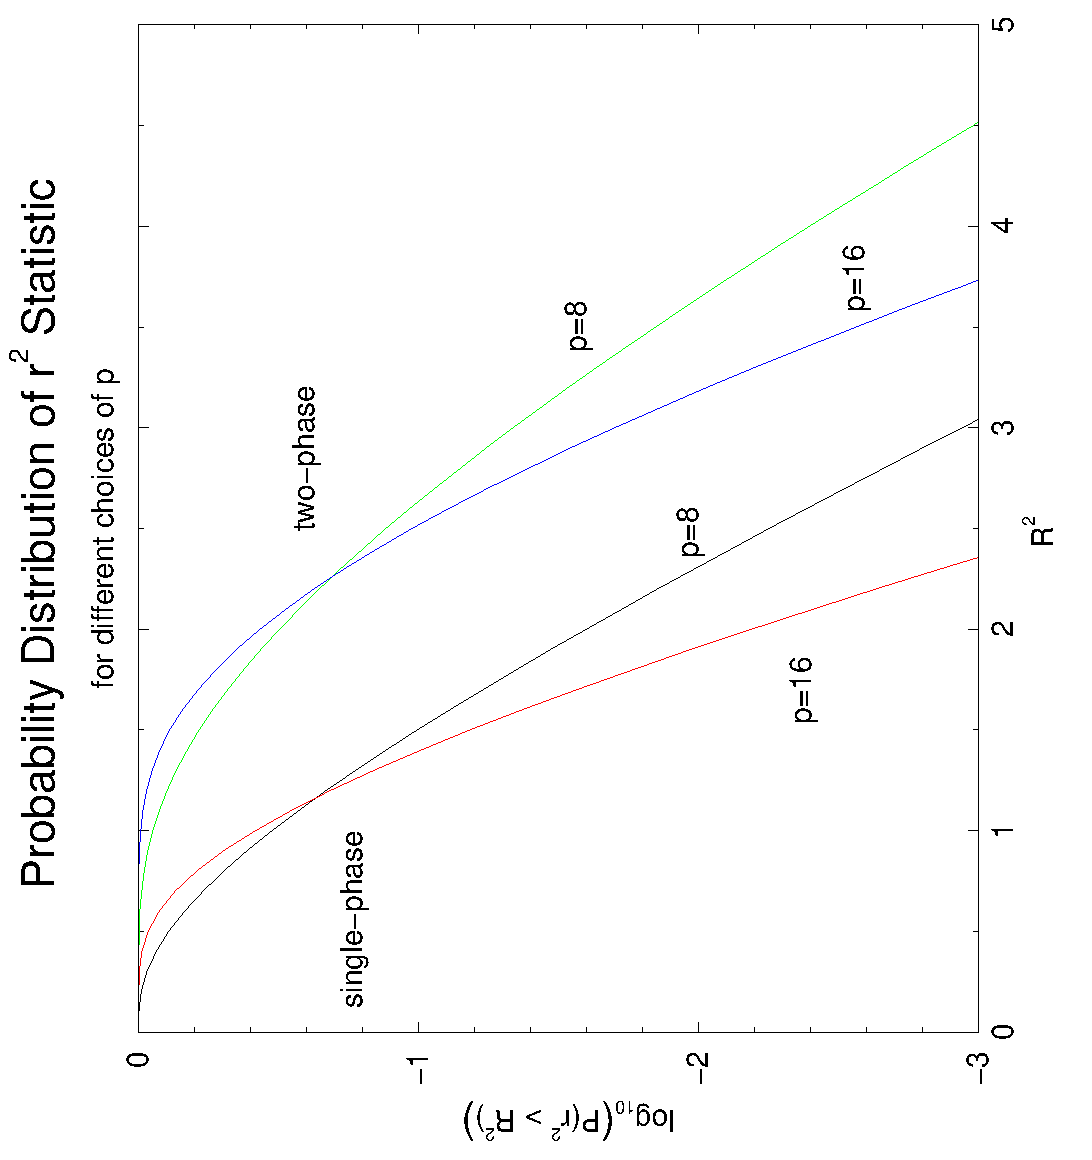
\epsfig{file=Figures/rsquared.eps,angle=-90,width=4in}
\index{colorpage}
\caption{ \label{f:rsquared}
The probability that the $r^2$ statistic exceeds a given threshold $R^2$
is shown for both the single-phase and two-phase test, for $p=8$ and
$p=16$ frequency ranges.  For example, for the single-phase $p=8$ test,
the probability that $r^2 > 2.31$ is 1\% for a chirp plus Gaussian noise.
For the single-phase test with $p=16$ the probability of exceeding the
same threshold is about $10^{-3}$.
}
\end{center}
\end{figure}

\clearpage

\subsection{ How does the $r^2$ test work ?}
In Section \ref{ss:veto} we have derived the statistical properties of
the $r^2$ test, and described it in mathematical terms.  This is a
bit deceptive, because this test was actually developed based on some
simple physical intuition.  We noticed with experience that many of the
high SNR events that were not found by the outlier {\tt is\_gaussian()}
test did not sound anything like chirps (when listened to with the {\tt
audio()} and {\tt sound()} functions).  It was clear from just listening
that for these spurious signals did not have the low frequency signal
arriving first, followed by the high frequency signal arriving last,
in the same way as a chirp signal.  So in fact the $r^2$ test was
designed to discriminate the way in which the different frequencies
arrived with time.  In effect, the filter used to construct the signal
$S_1$ passes only the lowest frequencies, the filter used to construct
the signal $S_2$ passes the next-to-lowest frequencies, and so on.
The filter which produces the signal $S_p$ passes the highest range of
frequencies which would make a significant contribution (i.e. a fraction
$1/p$) of the SNR for a true chirp.

If the signal is a true chirp, then the outputs of each of these different
filters (the $S_i(t_0)$ may be thought of as functions of lag $t_0$)
all peak at the same time-offset $t_0$, the {\it same} time-offset that
maximizes the total signal $S(t_0)$.  This is illustrated in Figure \ref{f:timefreqplot}.
\begin{figure}[h]
\begin{center}
\epsfig{file=Figures/filter3.eps,width=4in,angle=-90}
\index{colorpage}
\caption{
\label{f:timefreqplot}
This figure shows the output of four single-phase filters for the $p=4$
case, for a ``true chirp" injected into a stream of real IFO data
(left set of figures) and a transient noise burst already present in
another stream of real IFO data (right set of figures). When a true
chirp is present, the filters in the different frequency bands all peak
at the same time offset $t_0$: the time offset which maximizes the SNR.
At this instant in time, all of the $S_i$ are about the same value.
However when the filter was triggered by a non-chirp signal, the filters
in the different frequency bands peak at different times, and in fact
at time $t_0$ they have very different values (some large, some small,
and so on).
}
\end{center}
\end{figure}
It is also instructive to compare the values of the filter
outputs (single-phase test) for the two cases shown in Figure
\ref{f:timefreqplot}.  For the injected chirp, the signal-to-noise ratio
was 9.2, and the signal values in the different bands were
\begin{eqnarray}
\nonumber
S_1 & = & 2.25\\
\nonumber
S_2 & = & 2.44\\
\nonumber
S_3 & = & 1.87\\
\nonumber
S_4 & = & 2.64\\
S & = & S_1 + S_2 + S_3 + S_4 = 9.2 \\
\nonumber
r^2 & = & \sum_{i=1}^4 (S/4 - S_i)^2 = 0.324\\
\nonumber
P & = & Q(3/2, 2 r^2) = 0.730,
\end{eqnarray}
so there is a large probability $P$ of having $r^2$ this large.

For the spurious noise event shown in Figure \ref{f:timefreqplot} the
SNR was quite similar (8.97) but the value of $r^2$ is very different:
\begin{eqnarray}
\nonumber
S_1 & = & 0.23\\
\nonumber
S_2 & = & 0.84\\
\nonumber
S_3 & = & 5.57\\
\nonumber
S_4 & = & 2.33\\
S & = & S_1 + S_2 + S_3 + S_4 = 8.97\\
\nonumber
r^2 & = & \sum_{i=1}^4 (S/4 - S_i)^2 = 17.1\\
\nonumber
P & = & Q(3/2, 2 r^2) =9.4 \times 10^{-15},
\end{eqnarray}
so the probability that this value of $r^2$ would be obtained for a chirp
plus Gaussian noise is extremely small.
\clearpage

\subsection{Function: {\tt splitup()}}
\label{ss:splitup}
\setcounter{equation}0
{\tt void splitup(float *working, float template, float *r, int n, float total, int p, int *indices)}\\
This routine takes as inputs a template and a noise-power spectrum, and
splits up the frequency spectrum into a set of sub-intervals to use
with the vetoing technique just described.

The arguments are:
\begin{description}
\item{\tt working:} Input.  An array {\tt working[0..n-1]} used for working space.
\item{\tt template:} Input.  The array {\tt template[0..n-1]} contains the positive
  frequency ($f \ge 0$) part of the complex function $\tilde T(f)$.
  The packing of $\tilde T$ into this array follows the scheme used by
  the {\it Numerical Recipes} routine {\tt realft()}, which is
  described between equations (12.3.5) and (12.3.6) of \cite{NumRec}.
  The DC component $\tilde T(0)$ is real, and located in {\tt template[0]}.
  The Nyquist-frequency component $\tilde T(f_{\rm Nyquist})$ is also
  real, and is located in {\tt template[1]}.  The array elements {\tt template[2]}
  and {\tt template[3]} contain the real and imaginary parts, respectively, of
  $\tilde T(\Delta f)$ where $\Delta f = 2 f_{\rm Nyquist}/n = (n
  \Delta t)^{-1}$.   Array elements {\tt template[2j]} and {\tt template[2j+1]}
  contain the real and imaginary parts of $\tilde T( j \; \Delta f)$
  for $j=1,\cdots,n/2-1$. 
\item{\tt r}: Input.  The array {\tt r[0..n/2]} contains the values of
  the real function $\tilde r$ which is twice the inverse of the receiver noise, as
  in equation (\ref{e:lag}), so that $\tilde r(f) = 2/\tilde
  S_h(|f|)$.  The array elements are arranged in order of increasing
  frequency, from the DC value at subscript 0, to the Nyquist frequency
  at subscript n/2.  Thus, the $j$'th array element {\tt r[j]} contains
  the real value $\tilde r(j \; \Delta f)$, for $j=0,1,\cdots,n/2$.
  Again it is assumed that $\tilde r(-f) = \tilde r^*(f) = \tilde r(f)$.
\item{\tt n}: Input.  The total length of the complex arrays
  {\tt template} and {\tt working}, and the number of points in the output
  array {\tt s}.  Note that the array {\tt r} contains $n/2+1$
  points.  n must be even.
\item{\tt total:} Input.  This is the total value of the integrated
  template squared over $S_h$; the frequency
  subintervals are choose so that each of the {\tt p} subintervals
  contains $1/p$ of this total.
\item{\tt p:} Input.  The number of frequency bands into which you want to divide the range
  from DC to $f_{\rm Nyquist}$.
\item{\tt indices:} Ouput.  The frequency bins of the first frequency band are
  {\tt i=0..indices[0]}.  The next frequency band is  {\tt i=indices[0]+1..indices[1]}.
  The {\tt p}'th frequency band is {\tt i=indices[p-2]+1..indices[p-1]}.
  Note that {\tt indices[p-1]=n-1}.
\end{description}
\begin{description}
\item{Author:}
Bruce Allen, ballen@dirac.phys.uwm.edu
\item{Comments:}
None.
\end{description}
\clearpage

\subsection{Function: {\tt splitup\_freq()}}
\label{ss:splitup_freq}
\setcounter{equation}0
{\tt float splitup\_freq(float c0, float c90, float *chirp0,  float
*chirp90, float norm, float* twice\_inv\_noise, int n, int offset, int
p, int* indices, float* stats, float* working, float* htilde)}\\
This routine returns the value of the statistic $r^2=\sum_{i=1}^p (\Delta S_i)^2$.  This is
a less-efficient version, which internally constructs filters for each of the different frequency
subintervals, and then filters the metric perturbation through those filters.  It is useful
to understand how the different frequency components behave in the time domain, after filtering.

The arguments are:
\begin{description}
\item{\tt c0:} Input.  The coefficient of the 0-phase template.
\item{\tt c90:} Input.  The coefficient of the $90^\circ$-phase template.  Note that
    $c_0^2 + c_{90}^2$ should be 1.
\item{\tt chirp0:} Input.  An array {\tt chirp0[0..n-1]} containing the FFT of the 0-phase chirp.
\item{\tt chirp90:} Input.  An array {\tt chirp90[0..n-1]} containing the FFT of the $90^\circ$-phase chirp.
\item{\tt norm:} Input.  The normalization of the 0-phase chirp.
\item{\tt twice\_inv\_noise:} Input.  The array {\tt twice\_inv\_noise[0..n/2]} contains $2/S_h(f)$,
   as described previously.
The array element {\tt twice\_inv\_noise[0]} contains
   the DC value, and the array element {\tt twice\_inv\_noise[n/2]}
   contains the value at the Nyquist frequency.
\item{\tt n:} Input.  Defines the lengths of the previous arrays.
\item{\tt offset:} Input.  The offset of the moment of maximum signal in the filter output.
\item{\tt p:} Input.  The number of frequency bands $p$ for the vetoing test.
\item{\tt indices:} Output.  An array {\tt indices[0..p-1]} used for internal storage of the
   frequency subintervals (see {\tt splitup()}.
\item{\tt stats:} Output.  An array {\tt stats[0..p-1]} containing the values of the $S_i$ for $i=1,\cdots,p$.
\item{\tt working:} Output.  An array {\tt working[0..n-1]} used for internal storage.
\item{\tt htilde:} Input.  An array {\tt htilde[0..n-1]} containing the positive frequency part of
  $\tilde h(f)$.
\end{description}
\begin{description}
\item{Author:}
Bruce Allen, ballen@dirac.phys.uwm.edu
\item{Comments:}
None.
\end{description}
\clearpage

\subsection{Function: {\tt splitup\_freq2()}}
\label{ss:splitup_freq2}
\setcounter{equation}0
{\tt float splitup\_freq2(float c0, float c90, float *chirp0,  float
*chirp90, float norm, float* twice\_inv\_noise, int n, int offset, int
p, int* indices, float* stats, float* working,float* htilde)}\\
This routine returns the value of the statistic $r^2=\sum_{i=1}^p
(\Delta S_i)^2$.  This is a more computationally-efficient version,
which does not filter $\tilde h$ through each of the $p$ independent
time domain filters.  The arguments are identical to those of {\tt splitup\_freq()}.

The arguments are:
\begin{description}
\item{\tt c0:} Input.  The coefficient of the 0-phase template.
\item{\tt c90:} Input.  The coefficient of the $90^\circ$-phase template.  Note that
    $c_0^2 + c_{90}^2$ should be 1.
\item{\tt chirp0:} Input.  An array {\tt chirp0[0..n-1]} containing the FFT of the 0-phase chirp.
\item{\tt chirp90:} Input.  An array {\tt chirp90[0..n-1]}
containing the FFT of the $90^\circ$-phase chirp.
\item{\tt norm:} Input.  The normalization of the 0-phase chirp.
\item{\tt twice\_inv\_noise:} Input.  The array {\tt twice\_inv\_noise[0..n/2]} contains $2/S_h(f)$,
   as described previously.
The array element {\tt twice\_inv\_noise[0]} contains
   the DC value, and the array element {\tt twice\_inv\_noise[n/2]}
   contains the value at the Nyquist frequency.
\item{\tt n:} Input.  Defines the lengths of the previous arrays.
\item{\tt offset:} Input.  The offset of the moment of maximum signal in the filter output.
\item{\tt p:} Input.  The number of frequency bands $p$ for the vetoing test.
\item{\tt indices:} Output.  An array {\tt indices[0..p-1]} used for internal storage of the
   frequency subintervals (see {\tt splitup()}.
\item{\tt stats:} Output.  An array {\tt stats[0..p-1]} containing the values of the $S_i$ for $i=1,\cdots,p$.
\item{\tt working:} Output.  An array {\tt working[0..n-1]} used for internal storage.
\item{\tt htilde:} Input.  An array {\tt htilde[0..n-1]} containing the positive frequency part of
  $\tilde h(f)$.
\end{description}
\begin{description}
\item{Author:}
Bruce Allen, ballen@dirac.phys.uwm.edu
\item{Comments:}
None.
\end{description}
\clearpage


\subsection{Function: {\tt splitup\_freq3()}}
\setcounter{equation}0
{\tt float splitup\_freq2(float c0, float c90, float *chirp0, float
*chirp90, float norm, float* twice\_inv\_noise, int n, int offset, int p,
int* indices, float* stats, float* working,float* htilde)}\\
This routine implements the two-phase $r^2$ statistic test.  It returns
the value of the statistic $r^2=\sum_{i=1}^p |\Delta S_i|^2$ as defined
in Eq.~(\ref{e:deftwhophaser2}).  It is algorithmically similar to {\tt
splitup\_freq2()},  except that it allows for the case where the phase
of the signal is unknown.  The arguments are identical to those of {\tt
splitup\_freq2()} but the array {\tt stats} has $2p$ elements since the
signals are complex.

Note: The GRASP library includes two additional functions which are
operationally identical to {\tt splitup\_freq3()}, called
{\tt splitup\_freq4()} and {\tt splitup\_freq5()}.  The last of
these is currently the most efficient implementation of the two-phase
$r^2$ test.  All the arguments of {\tt splitup\_freq[3-5]()} are
{\it identical}.

The arguments are:
\begin{description}
\item{\tt c0:} Input.  Used in the same way as in {\tt splitup\_freq2()}. 
\item{\tt c90:} Input.  Used in the same way as in {\tt splitup\_freq2()}.  Note that
 if templates have unit norm you can set $c_0^2 + c_1^2 = 4$.
\item{\tt chirp0:} Input.  An array {\tt chirp0[0..n-1]} containing 
the FFT of the 0-phase chirp.
\item{\tt chirp90:} Input.  An array {\tt chirp90[0..n-1]}
containing the FFT of the $90^\circ$-phase chirp.
\item{\tt norm:} Input.  The normalization of the 0-phase chirp.
\item{\tt twice\_inv\_noise:} Input.  The array {\tt
twice\_inv\_noise[0..n/2]} contains $2/S_h(f)$, as described previously.
The array element {\tt twice\_inv\_noise[0]} contains the DC value,
and the array element {\tt twice\_inv\_noise[n/2]} contains the value 
at the Nyquist frequency.
\item{\tt n:} Input.  Defines the lengths of the previous arrays.
\item{\tt offset:} Input.  The offset of the moment of maximum signal 
in the filter output.
\item{\tt p:} Input.  The number of frequency bands $p$ for the vetoing test.
\item{\tt indices:} Output.  An array {\tt indices[0..p-1]} used for
internal storage of the frequency subintervals (see {\tt splitup()}.
\item{\tt stats:} Output.  An array {\tt stats[0..2p-1]} containing
the real and imaginary parts of the $S_i$ for $i=1,\cdots,p$.
\item{\tt working:} Output.  An array {\tt working[0..n-1]} used for 
internal storage.
\item{\tt htilde:} Input.  An array {\tt htilde[0..n-1]} containing 
the positive frequency part of $\tilde h(f)$.
\end{description}
\begin{description}
\item{Authors}
Bruce Allen, ballen@dirac.phys.uwm.edu,
and Patrick Brady,  patrick@tapir.caltech.edu,
and Jolien Creighton jolien@tapir.caltech.edu.
\item{Comments:}
None.
\end{description}
\clearpage

\subsection{Example: {\tt optimal} program}
\setcounter{equation}0
This program reads the 40-meter data stream, and then filters it though
a chirp template corresponding to a pair of inspiraling $1.4 M_\odot$
neutron stars.

The correspondence between different arrays in this program, and the
quantities discussed previously in this section, is given below.  In these
equations, $\Delta t = 1/{\tt srate}$ is the sample time in seconds, and
$\Delta f = (n \Delta t)^{-1} = {\tt srate/npoint}$ is the size of a
frequency bin, in Hz.  Here $n={\tt npoint}$ is the number of points in
the data stream which are being optimally filtered in one pass.

Chirp templates (in frequency space) for the two polarizations are
related to the arrays \hbox{\tt chirp0[ ]} and \hbox{\tt chirp1[ ]} by
\begin{eqnarray}
\tilde T_{0}(f) &=& {\Delta t  \over {\tt HSCALE}} \;{\tt chirp0[\;]}\\
\tilde T_{90}(f) &=& {\Delta t \over {\tt HSCALE}} \; {\tt chirp1[\;]}
\end{eqnarray}
where the elements {\tt chirp0[2j]} and {\tt chirp0[2j+1]} are the real
and imaginary parts at frequency $f= j \Delta f$ (with the exception of
the Nyquist frequency, stored in {\tt chirp0[1]}).  Note that to ensure
that quantities within the code remain within the dynamic range of
floating point numbers, we have scaled up the template strain by a
constant factor {\tt HSCALE}; we also scale up the interferometer
output by the same factor, so that all program output (such as
signal-to-noise ratios) is independent of the value of {\tt HSCALE}.
If you're not comfortable with this, go ahead and change {\tt HSCALE} to 1.
It won't change anything, provided that you don't overflow the dynamic
range of the floating point variables!
The scaled interferometer response function is
\begin{equation}
{\tt response[\;]} = {\tt HSCALE}/{\tt ARMLENGTH} \times R(f),
\end{equation}
where the function $R(f)$ is defined by equation (\ref{e:rdef}).
The Fourier transform $\tilde h$ of the dimensionless strain is
obtained by multiplying $\Delta t$ and the FFT of {\tt channel.0} by
{\tt response[ ]}, yielding
\begin{equation}
\tilde h(f) = {\Delta t \over {\tt HSCALE}} {\tt htilde[\;]}.
\end{equation}
The one-sided noise power spectrum $S_h(f)$ is the average of 
\begin{equation}
S_h(f) = {2 \over n \Delta t} | \tilde h(f) |^2 =
{2 \over n \Delta t} {(\Delta t)^2 \over {\tt HSCALE}^2} |{\tt htilde[\;]}|^2
= {2 \Delta t \over n \; {\tt HSCALE}^2} |{\tt htilde[\;]}|^2.
\end{equation}
The power spectrum $S_h(f)$ is averaged using the same exponential
averaging technique described for the routine {\tt avg\_spec()}.  This
average is stored as
\begin{equation}
{  S_h(f)} = {2 \Delta t \over n \; {\tt HSCALE}^2 }
\langle |{\tt htilde[\;]}|^{2} \rangle 
= { \Delta t \over n \; {\tt HSCALE}^2 } {\tt mean\_pow\_spec[\;]}
\end{equation}
Twice the inverse of this average is stored in the array {\tt
twice\_inv\_noise[ ]}, so that
\begin{equation}
{2 \over S_h(f)} = { n \; {\tt HSCALE}^2 \over \Delta t} \; {\tt twice\_inv\_noise[\;]}.
\end{equation}
The expected noise-squared for the plus polarization is given by
equation (\ref{e:n2}):
\begin{eqnarray*}
\langle N^2 \rangle &=& {1 \over 2} (Q,Q)  = {1 \over 2} \int_{-\infty}^\infty df\;
{| \tilde T_{0}(f)|^2 \over S_h(f)} \\
&=&
{1 \over 2} {1 \over n \Delta t} FFT^{-1}_0 \left[
 {(\Delta t)^2 \over {\tt HSCALE}^2}  |{\tt chirp0[\;]} |^2 
{n {\tt HSCALE}^2 \over \Delta t} {1 \over 2} {\tt twice\_inv\_noise[\; ] } \right] \\
& = & {1 \over 2} FFT^{-1}_0 \left[ |{\tt chirp0[\;]} |^2 {1 \over 2} {\tt twice\_inv\_noise[\; ] } \right] \\
& \rightarrow & {1 \over 2} {\tt
correlate(\cdots,chirp0[\;],chirp0[\;],twice\_inv\_noise[\;],npoint)}.
\end{eqnarray*}
where the subscript on the inverse FFT means ``at zero lag", and
``$\rightarrow f$" means ``returned by the call to the function f".  We
have chosen a distance for the system producing the ``chirp" $\tilde
T_(f)$ so that the expected value of $\langle N^2 \rangle=1$.

In similar fashion, the signal $S$ at lag $t_0 $ is given
by
\begin{eqnarray}
   \nonumber
S  & = & ({\tilde h \over S_h}, \tilde Q) \\
    \nonumber
    & = & \int_{-\infty}^\infty df\;
       {\tilde h(f) \tilde T^*_{0}(f)  \over S_h(f)} \;
       {\rm e}^{-2 \pi i f t_0} \\
   \nonumber
   & = & {1 \over n \Delta t} FFT^{-1}_{i}\left[ {\Delta t \over {\tt
       HSCALE}} {\tt htilde[\;]} {\Delta t  \over {\tt HSCALE}} \;
       \left( {\tt chirp0[\;]} \right)^* { n \; {\tt HSCALE}^2 \over
       \Delta t } \; {1 \over 2} {\tt twice\_inv\_noise[\;]} \right] \\
\nonumber
   & = & FFT^{-1}_{i} \left[ {\tt htilde[\;]} \; {\tt chirp0[\;]} \;
   {1 \over 2} {\tt twice\_inv\_noise[\;]} \right]\\
& \rightarrow & {\tt
correlate(\cdots,htilde[\;],chirp0[\;],twice\_inv\_noise[\;],npoint)},
\end{eqnarray}
where now the subscript on the FFT means ``at lag $t = i \; \Delta t$".

You might wonder why we have been so careful -- after all, both the
signal and the noise, as we've defined them, are dimensionless, so it's
not surprising that all of the factors of $\Delta t$ drop out of the
final formulae for the signal and the expected noise-squared.  The main
reason we've been so long winded is to show exactly how the units cancel out,
and to demonstrate that there aren't any missing dimensionless constants,
like {\tt npoint}, left out of the program.  Some sample output from
this program is shown in the next section.
\clearpage
\lgrindfile{Includes/optimal.tex}
\clearpage

\subsection{Some output from the {\tt optimal} program}
Some output from the {\tt optimal} program follows:
\begin{verbatim}
...
max snr: 3.11 offset: 23623 data start: 180.00 sec. variance: 0.94044
max snr: 2.91 offset: 3311 data start: 185.17 sec. variance: 0.84484
...
max snr: 2.53 offset: 19041 data start: 309.26 sec. variance: 0.70333
max snr: 2.98 offset: 35711 data start: 314.43 sec. variance: 0.67523

Max SNR: 8.71 (offset 42109) variance 0.805030
   If impulsive event, offset 55624 or time 325.23
   If inspiral, template start offset 42109 (time 323.86) coalescence time 325.23
   Normalization: S/N=1 at 116.75 kpc
   Linear combination of max SNR: 0.9315 x phase_0 + 0.3638 x phase_pi/2
   Less than 1% probability that this is a chirp (p=0.000000).
   Distribution: s= 23, N>3s= 12 (expect 176), N>5s= 0 (expect 0)
   Distribution does not appear to have outliers...

max snr: 2.51 offset: 31183 data start: 324.77 sec. variance: 0.63028
max snr: 2.56 offset: 49909 data start: 329.94 sec. variance: 0.66853
...
max snr: 2.82 offset: 35080 data start: 3002.03 sec. variance: 0.77306
max snr: 2.61 offset: 33141 data start: 3007.20 sec. variance: 0.74268

Max SNR: 89.75 (offset 16678) variance 82.547005
   If impulsive event, offset 30193 or time 3015.43
   If inspiral, template start offset 16678 (time 3014.06) coalescence time 3015.43
   Normalization: S/N=1 at 128.49 kpc
   Linear combination of max SNR: -0.3955 x phase_0 + 0.9185 x phase_pi/2
   Less than 1% probability that this is a chirp (p=0.000000).
   Distribution: s= 29, N>3s= 157 (expect 176), N>5s= 30 (expect 0)
   Distribution has outliers! Reject

max snr: 3.24 offset: 22412 data start: 3017.54 sec. variance: 0.99474
max snr: 2.73 offset: 37777 data start: 3022.71 sec. variance: 0.75325
...
max snr: 2.80 offset: 5893 data start: 4140.89 sec. variance: 0.73240
max snr: 2.75 offset: 46932 data start: 4146.06 sec. variance: 0.69654

Max SNR: 6.08 (offset 30002) variance 0.883380
   If impulsive event, offset 43517 or time 4155.64
   If inspiral, template start offset 30002 (time 4154.27) coalescence time 4155.64
   Normalization: S/N=1 at 113.04 kpc
   Linear combination of max SNR: -0.4773 x phase_0 + 0.8787 x phase_pi/2
   POSSIBLE CHIRP!  with > 1% probability (p=0.024142).
   Distribution: s= 31, N>3s= 399 (expect 176), N>5s= 53 (expect 0)
   Distribution has outliers! Reject

max snr: 2.77 offset: 15985 data start: 4156.40 sec. variance: 0.72095
max snr: 2.69 offset: 47338 data start: 4161.57 sec. variance: 0.69708
...
\end{verbatim}
This output shows three events that triggered an optimal filtering
routine.  The first and second of these events were rejected for
different reasons.  The first was rejected because if failed the
frequency-distribution test.  The second was rejected because it had 30
outlier points.  The third failed for the same reason: it had 53
outlier points.

Next, we show some output when a fake chirp signal is injected into the data stream.  This
can be done for example by modifying {\tt optimal} to read:
\begin{verbatim}
invMpc_inject=100.0;   /* To inject a signal at 10 kpc, set this to 100.0 */
time_inject_chirp(1.0,0.0,12345,invMpc_inject,chirp0,chirp90,data,response,output0,npoint);
\end{verbatim}
This produces the following output:
\begin{verbatim}
...
Max SNR: 9.96 (offset 12345) variance 0.872624
   If impulsive event, offset 25860 or time 187.79
   If inspiral, template start offset 12345 (time 186.42) coalescence time 187.79
   Normalization: S/N=1 at 152.17 kpc
   Linear combination of max SNR: 0.9995 x phase_0 + -0.0304 x phase_pi/2
   POSSIBLE CHIRP!  with > 1% probability (p=0.421294).
   Distribution: s= 23, N>3s= 12 (expect 176), N>5s= 0 (expect 0)
   Distribution does not appear to have outliers...


Max SNR: 12.84 (offset 12345) variance 0.834527
   If impulsive event, offset 25860 or time 192.96
   If inspiral, template start offset 12345 (time 191.59) coalescence time 192.96
   Normalization: S/N=1 at 132.47 kpc
   Linear combination of max SNR: 0.9953 x phase_0 + 0.0973 x phase_pi/2
   POSSIBLE CHIRP!  with > 1% probability (p=0.949737).
   Distribution: s= 22, N>3s= 28 (expect 176), N>5s= 0 (expect 0)
   Distribution does not appear to have outliers...


Max SNR: 14.86 (offset 12345) variance 0.801640
   If impulsive event, offset 25860 or time 198.13
   If inspiral, template start offset 12345 (time 196.76) coalescence time 198.13
   Normalization: S/N=1 at 127.90 kpc
   Linear combination of max SNR: 0.9993 x phase_0 + -0.0372 x phase_pi/2
   POSSIBLE CHIRP!  with > 1% probability (p=0.999236).
   Distribution: s= 22, N>3s= 35 (expect 176), N>5s= 0 (expect 0)
   Distribution does not appear to have outliers...
...
\end{verbatim}
The code is correctly finding the chirps, getting the distance and phase and
time location of the chirps about as accurately as one would expect given
the level of the IFO noise.

There are several interesting lessons that one can learn from this
optimal filtering experience.  The first is that (roughly speaking) the
events that trigger an optimal filter (driving the output to a value
much larger than would be expected for a colored-noise Gaussian input)
can be broken into two classes: those which can be seen in the raw data
stream, and those which can not.  Here, by ``seen in the raw data
stream", we mean ``visible to the naked eye upon examination of a
graph".  Shown in the following two figures are examples of each type
of spurious event.

\begin{figure}
\begin{center}
\epsfig{file=Figures/data.000.ps,angle=-90,bbllx=40pt,bblly=72pt,
bburx=580pt,bbury=720pt,width=4in}
\index{colorpage}
\caption{ \label{f:drip}
This shows the event that triggered the $2\times 1.4$ solar mass binary
inspiral filter with a SNR of 8.71 (see the first set of sample output
from the optimal filtering code above, at time 325.23).  This same
``event" can also be seen in Figure~\ref{f:diag0}.  The horizontal axis
is sample number, with samples $\approx 10^{-4}$ seconds apart; the
vertical axis is the raw (whitened) IFO output.  The event labeled
``drip" can be heard in the data (it sounds like a faucet drip) and is
picked up by the optimal filtering technique, but it is NOT visible to
the naked eye.  This event is vetoed by the splitup technique described
earlier - it has extremely low probability of being a chirp plus
stationary noise.}
\end{center}
\end{figure}

\begin{figure}
\begin{center}
\epsfig{file=Figures/data.001.ps,angle=-90,bbllx=40pt,bblly=72pt,
bburx=580pt,bbury=720pt,width=4in}
\index{colorpage}
\caption{ \label{f:bump1}
This another event that triggered the $2\times 1.4$ solar mass binary
inspiral filter with a SNR of 17.33.  This event sounds like a ``bump";
it is probably due to a bad cable connection.  It can be easily seen
(and vetoed) in the time domain.  A close-up of this is shown in the next
figure.}
\end{center}
\end{figure}

\begin{figure}
\begin{center}
\epsfig{file=Figures/data.001b.ps,angle=-90,bbllx=40pt,bblly=72pt,
bburx=580pt,bbury=720pt,width=4in}
\index{colorpage}
\caption{ \label{f:bump2}
A close-up of the previous graph, showing the structure of the ``bump".}
\end{center}
\end{figure}

\begin{figure}
\begin{center}
\epsfig{file=Figures/data.002.ps,angle=-90,bbllx=40pt,bblly=72pt,
bburx=580pt,bbury=720pt,width=4in}
\caption{ \label{f:scrape1}
This another event that triggered the $2\times 1.4$ solar mass binary
inspiral filter with a SNR of 32.77.  This event sounds like a shovel
scraping on the ground; its origin is unknown.  It can be easily seen
(and vetoed) in the time domain.}
\end{center}
\index{colorpage}
\end{figure}

\begin{figure}
\begin{center}
\epsfig{file=Figures/data.002b.ps,angle=-90,bbllx=40pt,bblly=72pt,
bburx=580pt,bbury=720pt,width=4in}
\caption{ \label{f:scrape2}
A close-up of the previous graph, showing the structure of the ``scrape".}
\end{center}
\end{figure}
\index{colorpage}
\clearpage

\clearpage
\subsection{The effective distance to which a source can be seen}
\label{ss:eff_distdef}
\par\noindent

Given a gravitational-wave detector with some known noise spectrum, it
would clearly be useful to define an ``effective distance'' $D_{\rm
eff}$ to which some given gravitational-wave source can be seen.  To
first order, any source located farther away from the detector than
$D_{\rm eff}$ would be too weak to be detectable in the datastream.
Sources closer than $D_{\rm eff}$ would be detectable.

This naive, heuristic picture of $D_{\rm eff}$ doesn't make much sense
in the real world because the source does not emit isotropically, and
the detector does not detect isotropically: there are positions on the
sky for which the detector can ``see'' farther, and the source
radiates more strongly into some angles than others.  A useful
definition of $D_{\rm eff}$ must therefore average over angles in a
meaningful, well-understood way.

One simple way to average over angles is to use Eq. (2.30) of Ref.\
{\cite{flanhughes1}}.  In that reference, Flanagan and Hughes show
that the signal-to-noise ratio, rms angle averaged over all source
orientations and all positions on the sky, depends only on the
spectrum of emitted gravitational-wave energy, $dE_{\rm gw}/df$.
Rearranging their formula (2.30) slightly, the effective distance to
which a source can be seen with some rms angle-averaged
signal-to-noise ratio $\rho_0$ is then
\begin{equation}
D^{\rm FH}_{\rm eff}(\rho_0)^2 = 
 {2(1+z)^2\over5\pi^2\rho_0^2}
\left( {G \over c^3} \right) \int_0^\infty df {1\over f^2 S_h(f)}{dE_{\rm gw}\over df}[(1+z)f]\;.
\label{eq:effdist_fh}
\end{equation}
The distance $D^{\rm FH}_{\rm eff}$ so defined is actually a
luminosity distance; assuming some set of cosmological parameters and
using standard formulae, one can then easily convert $D^{\rm FH}_{\rm
eff}$ to an effective redshift $z^{\rm FH}_{\rm eff}$, and thence
compute the comoving volume $V_c(z^{\rm FH}_{\rm eff})$ that is
contained to that distance.  If one assumes that the event rate of
sources locked into Hubble flow does not evolve with redshift, this
allows one to simply convert from an event rate density $R$ [with
units number/(Mpc$^3$ year)] to a detected event rate $N$ (with units
number/year).  (This assumption is clearly a rather bad one: the event
rate will undoubtedly evolve with redshift.  However, we don't
currently know {\it how} it will so evolve.  This simple, albeit
stupid, assumption is a useful one for estimating event rates for
gravitational-wave sources.)

Notice that the cosmological redshift $z$ explicitly appears in
Eq. (\ref{eq:effdist_fh}).  These factors enter in such a way that the
mass ``imprinted'' on the gravitational waveform ({\it i.e.}, the mass
that gravitational-wave detections measure at the earth) will be
redshift from $M$ to $(1+z)M$.

Finn and Chernoff {\cite{finnandchernoff}} define an effective
distance in a somewhat different and more careful manner.
Given a noise spectrum and given a threshold signal-to-noise ratio
$\rho_0$, they define an effective distance $D^{\rm FC}_{\rm
eff}(\rho_0)$ as
\begin{equation}
N(\rho > \rho_0)  = {4\pi\over3} D^{\rm FC}_{\rm eff}(\rho_0)^3 R\;.
\label{eq:effdist_fc}
\end{equation}
In words, the detection rate of events with signal-to-noise ratio
$\rho$ greater than the threshold $\rho_0$ is given the event rate
density in space $R$ times the volume of a sphere of radius $D^{\rm
FC}_{\rm eff}(\rho_0)$.  Finn and Chernoff then calculate $D^{\rm
FC}_{\rm eff}$ using Monte-Carlo integration; see
{\cite{finnandchernoff}} for details.

Thorne {\cite{thornetofinnhughes},\cite{thornefinnerror}} has shown
that for a pair of $1.4\,M_\odot-1.4\,M_\odot$ neutron stars {\it and}
for distances small enough that cosmological effects are negligible,
the definitions given in Eqs.\ (\ref{eq:effdist_fh}) and
(\ref{eq:effdist_fc}) are related by
\begin{equation}
{D^{\rm FC}_{\rm eff}\over D^{\rm FH}_{\rm eff}} = 1.10\;.
\label{eq:fudgefactor}
\end{equation}
For the purposes of GRASP, we will use an effective distance that is
based on (\ref{eq:effdist_fh}) because it is quick and simple to
calculate, but correct using (\ref{eq:fudgefactor}) in the hope that
this will put us in reasonable agreement with the very careful
calculations of Finn and Chernoff.  (This factor of $1.10$ probably
varies somewhat with total system mass and with cosmological effects.)
The formula for $D_{\rm eff}(\rho_0)$ that we use is
\begin{equation}
D_{\rm eff}(\rho_0)^2 = (1.10)^2 \times{2(1+z)^2\over5\pi^2
\rho_0^2}\int_0^\infty df {1\over f^2 S_h(f)}{dE_{\rm gw}
\over df}[(1+z)f]\;.
\label{eq:effdist}
\end{equation}

The following routine calculates this effective distance, providing
also the associated redshift and comoving volume.

\clearpage
\subsection{Function: {\tt inspiral\_dist()}}
\label{ss:inspiral_dist}
\begin{verbatim}
void inspiral_dist(double *deff, double *z, double *Vc, double m1_z,
                   double m2_z, double snr, double S_h[], int npoint,
                   double srate, double h100)
\end{verbatim}
\noindent
This function computes the effective distance to which a binary
inspiral with redshifted masses {\tt m1\_z} and {\tt m2\_z} can be
seen with the noise spectrum {\tt S\_h[]}.

It uses the energy spectrum
\begin{equation}
{dE_{\rm gw}\over df} = {\pi^{2/3} \over 3}\mu M^{2/3} f^{-1/3}
\label{eq:inspspec}
\end{equation}
to describe the inspiral for frequencies $f < f_{\rm merge} = 0.02/M$,
and zero above $f_{\rm merge}$ (as in reference {\cite{flanhughes1}}).
To convert from luminosity distance to redshift, it assumes a universe
flat cosmology ($\Lambda=0$, $\Omega=1$) with a Hubble constant $H_0 =
75\,{\rm km}/{{\rm Mpc}\,{\rm sec}}$, and uses an Eq. (11) from
{\cite{markovic}}.  To convert from redshift to comoving volume, it
uses Eq. (27) of {\cite{dwhogg}} or Eq. (2.56) with $q_0=1/2$ of
\cite{kolbturner}.

The arguments to the function are:
\begin{description}
\item{{\tt deff:}} Output.  The effective distance in megaparsecs.
\item{{\tt z:}} Output.  Redshift corresponding that effective distance.
\item{{\tt Vc:}} Output.  Comoving volume at the redshift in cubic
megaparsecs.
\item{{\tt m1\_z:}} Input.  Redshifted mass one, $(1+z)m_1$.
\item{{\tt m2\_z:}} Input.  Redshifted mass two, $(1+z)m_2$.
\item{{\tt snr:}} Input.  The signal-to-noise ratio at which the
effective distance is {\tt deff}.
\item{{\tt S\_h:}} Input.  The spectral density of noise in Hz$^{-1}$.
\item{{\tt npoint:}} Input.  The number of data points in {\tt S\_h}.
\item{{\tt srate:}} Input.  The sampling rate used to construct the
noise spectrum, Hz.
\item{{\tt h100:}} Input.  The Hubble constant in units of 100 km/sec/Mpc.
\end{description}

\begin{description}
\item{Author:} Scott Hughes, hughes@tapir.caltech.edu
\end{description}
     
\clearpage
\subsection{Function: {\tt merger\_dist()}}
\label{ss:merger_dist}
\begin{verbatim}
void merger_dist(double *deff, double *z, double *Vc, double m1_z,
                 double m2_z, double snr, double S_h[], int npoint,
                 double srate,double h100)
\end{verbatim}
\noindent
This function computes the effective distance to which a binary
merger with redshifted masses {\tt m1\_z} and {\tt m2\_z} can be
seen with the noise spectrum {\tt S\_h[]}.

It uses the energy spectrum
\begin{equation}
{dE_{\rm gw}\over df} = {\epsilon M\over f_{\rm qnr} - f_{\rm merge}}
\label{eq:mergspec}
\end{equation}
to describe the merger, using parameters $\epsilon = 0.1$, $f_{\rm
qnr} = 0.13/M$, $f_{\rm merge} = 0.02/M$ (as in reference
{\cite{flanhughes1}}).  As such it is, strictly speaking, only
applicable to binary black hole mergers.  Its operation is otherwise
identical to {\tt inspiral\_dist()}.

The arguments to the function are:
\begin{description}
\item{{\tt deff:}} Output.  The effective distance in megaparsecs.
\item{{\tt z:}} Output.  Redshift corresponding that effective distance.
\item{{\tt Vc:}} Output.  Comoving volume at the redshift in cubic
megaparsecs.
\item{{\tt m1\_z:}} Input.  Redshifted mass one, $(1+z)m_1$.
\item{{\tt m2\_z:}} Input.  Redshifted mass two, $(1+z)m_2$.
\item{{\tt snr:}} Input.  The signal-to-noise ratio at which the
effective distance is {\tt deff}.
\item{{\tt S\_h:}} Input.  The spectral density of noise in Hz$^{-1}$.
\item{{\tt npoint:}} Input.  The number of data points in {\tt S\_h}.
\item{{\tt srate:}} Input.  The sampling rate used to construct the
noise spectrum, Hz.
\item{{\tt h100:}} Input.  The Hubble constant in units of 100 km/sec/Mpc.
\end{description}

\begin{description}
\item{Author:} Scott Hughes, hughes@tapir.caltech.edu
\end{description}

\clearpage
\subsection{Example: {\tt compute\_dist} program}
\label{ss:compute_dist}

This program will tell you the distance to which a binary with given
redshifted masses [$(1+z)m_1,(1+z)m_2$] can be seen with a given
signal-to-noise rate in some given detector (which must be listed in
the GRASP file {\tt detectors.dat}).  It will also tell you the
redshift at that effective (luminosity) distance and the corresponding
comoving volume.  It uses that comoving volume to convert a given
event rate density to a measured event rate.

The code specifies its various input parameters with command line
flags.  Thus,\\
{\tt compute\_dist -m1 5 -m2 7 -snr 6 -d 24 -R 2.e-7 -h100 0.75}\\
will compute the effective distance for a binary that has $(1+z)m_1 =
5M_\odot$, $(1+z)m_2 = 7M_\odot$ with signal-to-noise ratio 6 in detector
24 (the zeroth stage of enhancement at the Livingston LIGO site); and it
will compute the detected event rate with an assumption that the event
rate density is $2\times10^{-7}$ events per cubic megaparsec per year,
in a cosmology with Hubble constant today of 75 km/sec/Mpc.  If a flag
or parameter is omitted, default values are used; type\\
{\tt compute\_dist -h}\\
 to see those default
values.
     
\lgrindfile{Includes/compute_dist.tex}

\begin{description}
\item{Author:} Scott Hughes, hughes@tapir.caltech.edu
\end{description}

